\section{Results}
\label{sec:results}

\subsection{Descriptive Trends}

Figure~\ref{fig:cs_share_full} plots the annual share of original FDA approvals classified as controlled substances from 1939 through 2025. Three features stand out. First, the share fluctuates broadly in the 5--15\% range over the full sample, with no visually obvious structural break at PDUFA (1992). Second, the series exhibits substantial year-to-year noise in the early portion of the sample, when annual approval counts were small. Third, a moderate elevation is visible from roughly 2009 to 2012, which Section~\ref{sec:results_spike} documents as a separable phenomenon.

\begin{figure}[htbp]
\centering
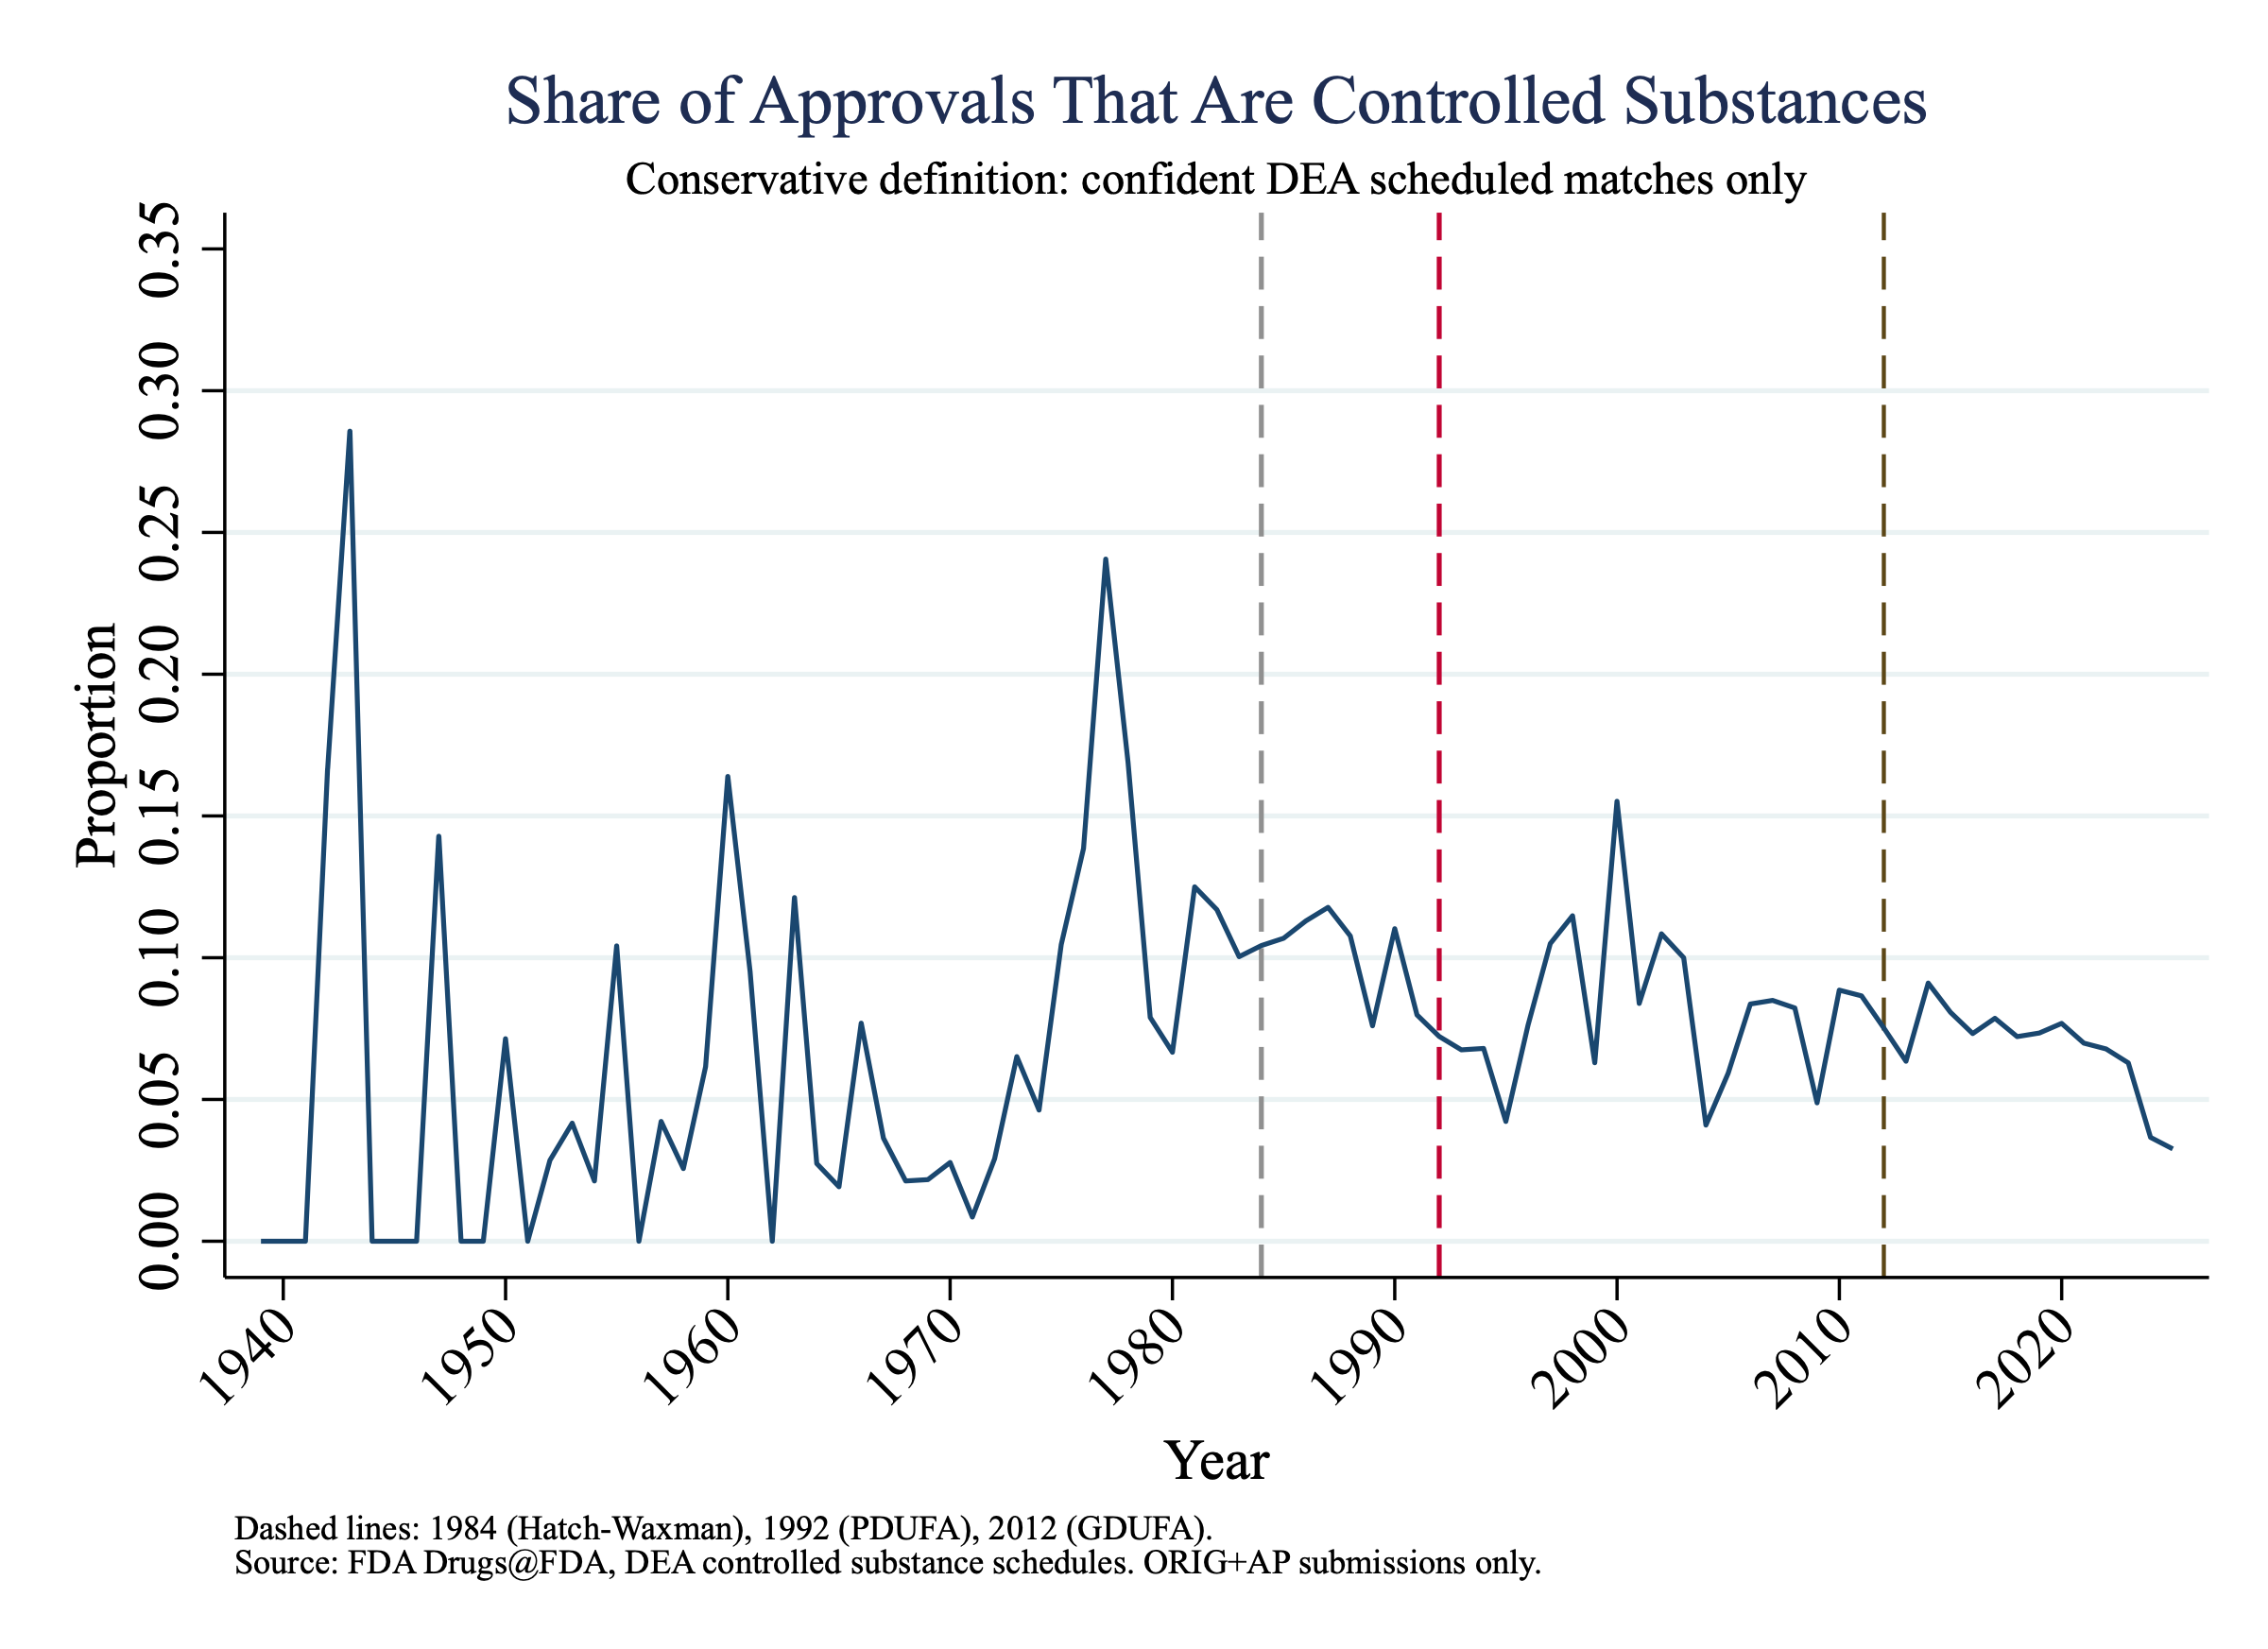
\includegraphics[width=0.92\textwidth]{../output/figures/stata/fig_cs_share.png}
\caption{Annual controlled-substance share of FDA original approvals, 1939--2025. Conservative definition: confident DEA scheduled matches only. Dashed vertical lines mark 1984 (Hatch--Waxman), 1992 (PDUFA), and 2012 (GDUFA).}
\label{fig:cs_share_full}
\end{figure}

Figure~\ref{fig:cs_share_by_type} disaggregates the CS share by application type. The NDA CS share fluctuates narrowly around 5--8\% throughout the sample with no visible trend break at PDUFA. The ANDA CS share is higher --- peaking near 20\% in the early 1980s --- and declines after Hatch--Waxman as the expansion in non-CS generic approvals dilutes the CS share. Years with fewer than five NDA or ANDA approvals are excluded to suppress noise.

\begin{figure}[htbp]
\centering
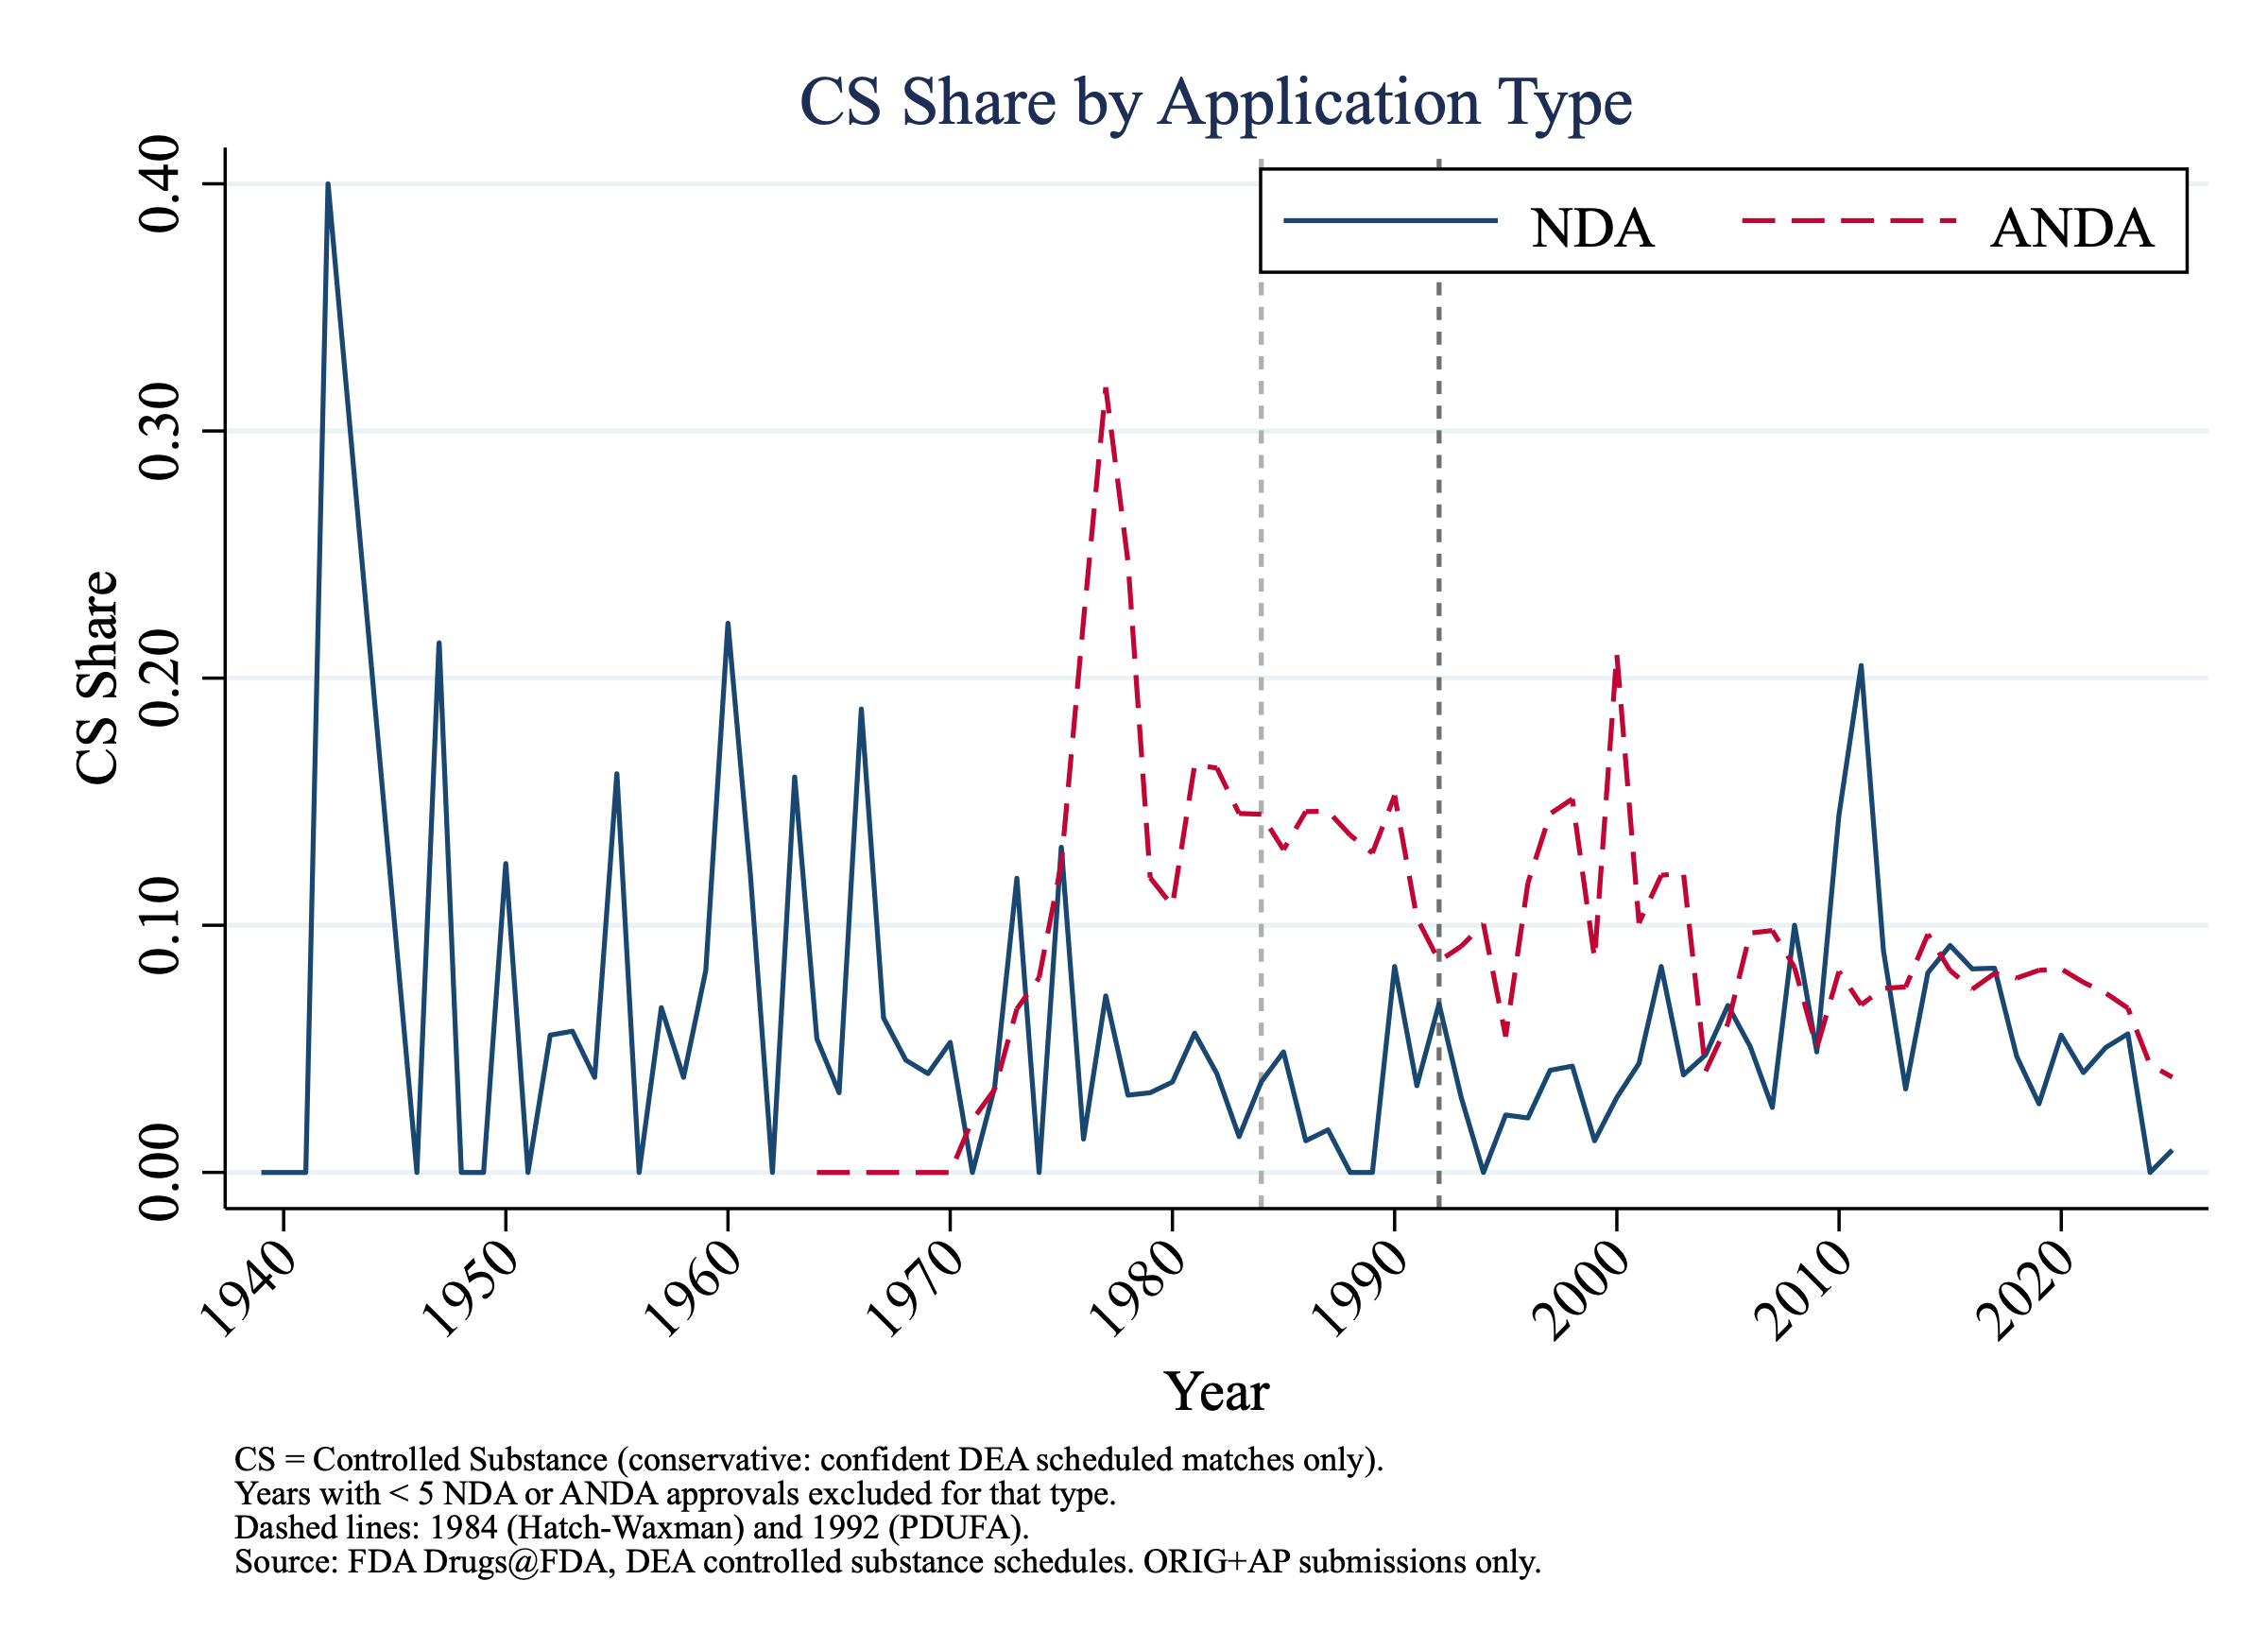
\includegraphics[width=0.92\textwidth]{../output/figures/stata/fig_cs_share_by_appltype.png}
\caption{Annual CS share by application type (NDA vs.\ ANDA), 1939--2025. Years with fewer than five NDA or ANDA approvals are excluded. Dashed lines as in Figure~\ref{fig:cs_share_full}.}
\label{fig:cs_share_by_type}
\end{figure}

\subsection{PDUFA Event Study: Full Sample}
\label{sec:results_pdufa_full}

Figure~\ref{fig:event_study_full} reports event-study point estimates and 95\% confidence intervals from the share-based ITS specification of equation~\ref{eq:its}, with event time measured in years relative to PDUFA (1992). Pre-policy estimates ($\tau < 0$) are clustered near zero, consistent with the parallel-trends assumption over the pre-PDUFA window. Post-policy estimates ($\tau > 0$) move modestly above and below zero with no clear level shift or trend break at $\tau = 0$. The confidence intervals are wide --- a feature of any single national time series --- but they are tight enough to bound the immediate post-1992 deviation from the pre-trend within roughly a percentage-point band.

\begin{figure}[htbp]
\centering
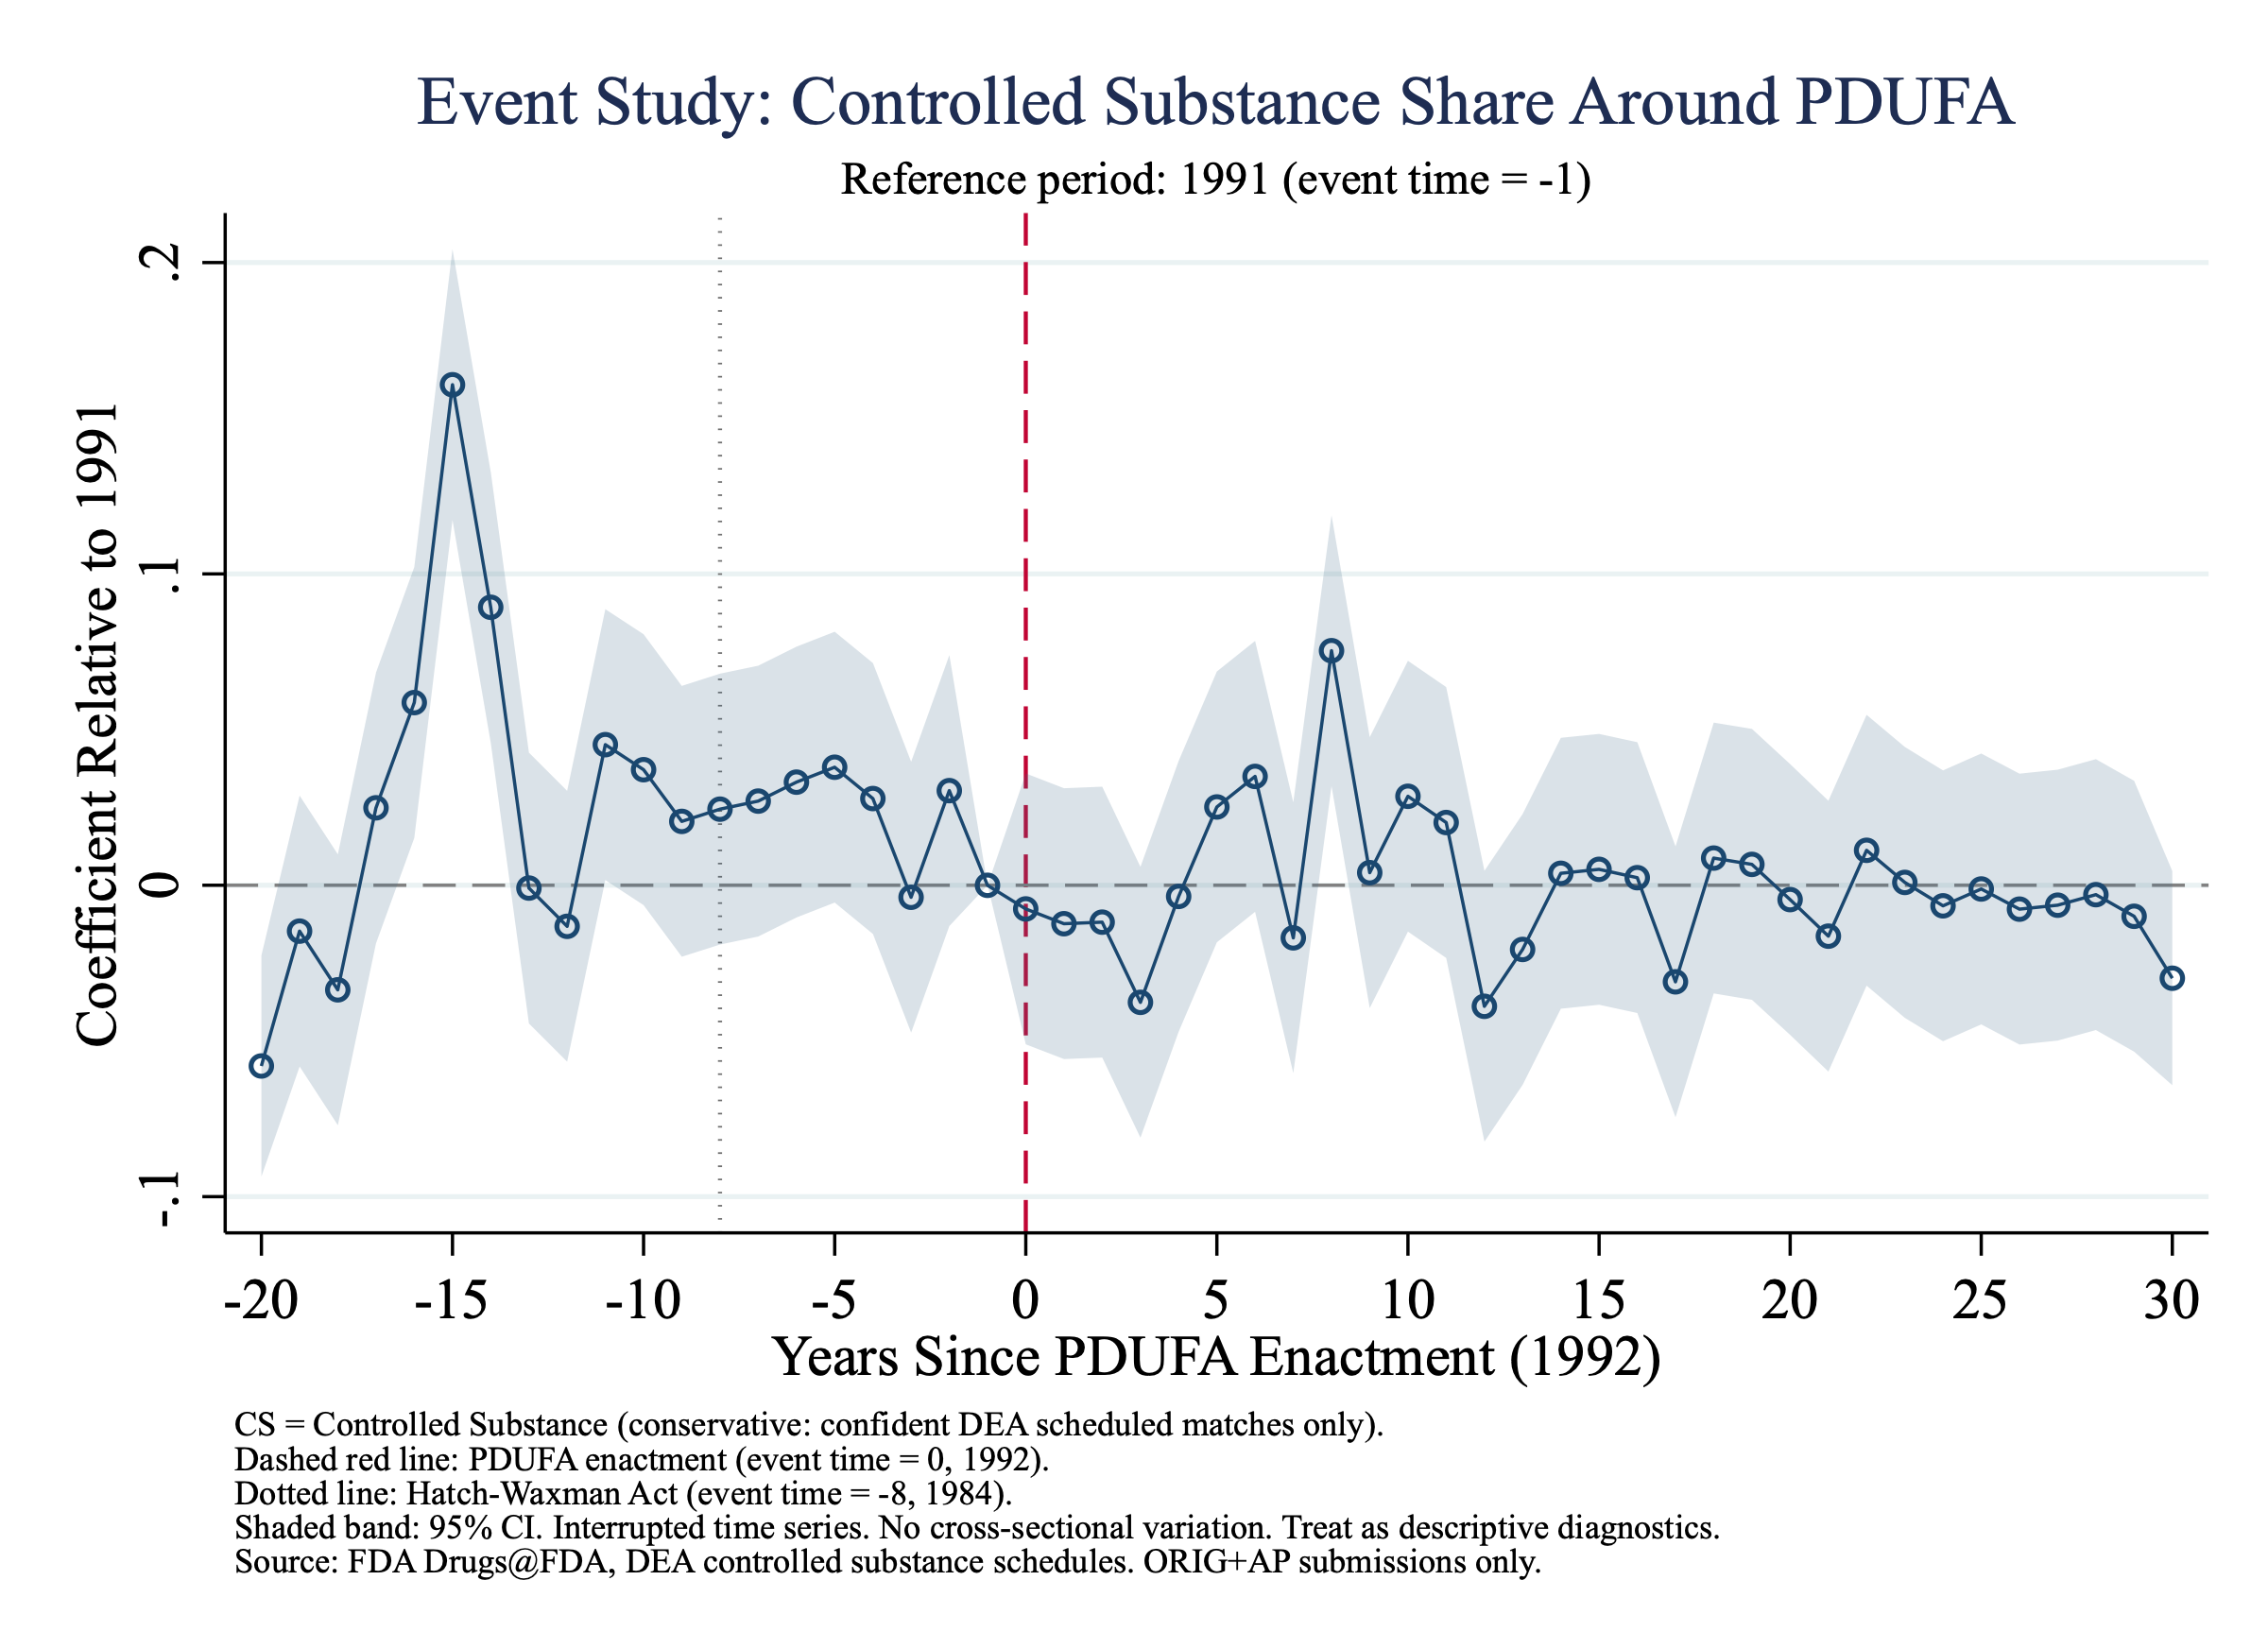
\includegraphics[width=0.92\textwidth]{../output/figures/stata/event_study_cs_share.png}
\caption{PDUFA event study: ITS coefficients on CS share. Event time 0 = 1992 (PDUFA enactment). Reference period: $\tau = -1$ (1991). End-caps at $[-20, +30]$. 95\% confidence intervals.}
\label{fig:event_study_full}
\end{figure}

\subsection{PDUFA Event Study: NDA-Only Sample}
\label{sec:results_nda}

Figure~\ref{fig:event_study_nda} restricts the event-study to new drug applications. This is the theoretically relevant subsample: PDUFA directly governs NDA review times and does not apply to ANDA submissions. The NDA CS share series is noisier than the pooled series because annual NDA counts are smaller, but the event-study profile reveals a feature that organizes the rest of the analysis: the largest positive deviations from the pre-trend occur around event times 17--19 (calendar years 2009--2011), not at or near $\tau = 0$. A composition response operating through the user-fee channel should appear near the policy date.

\begin{figure}[htbp]
\centering
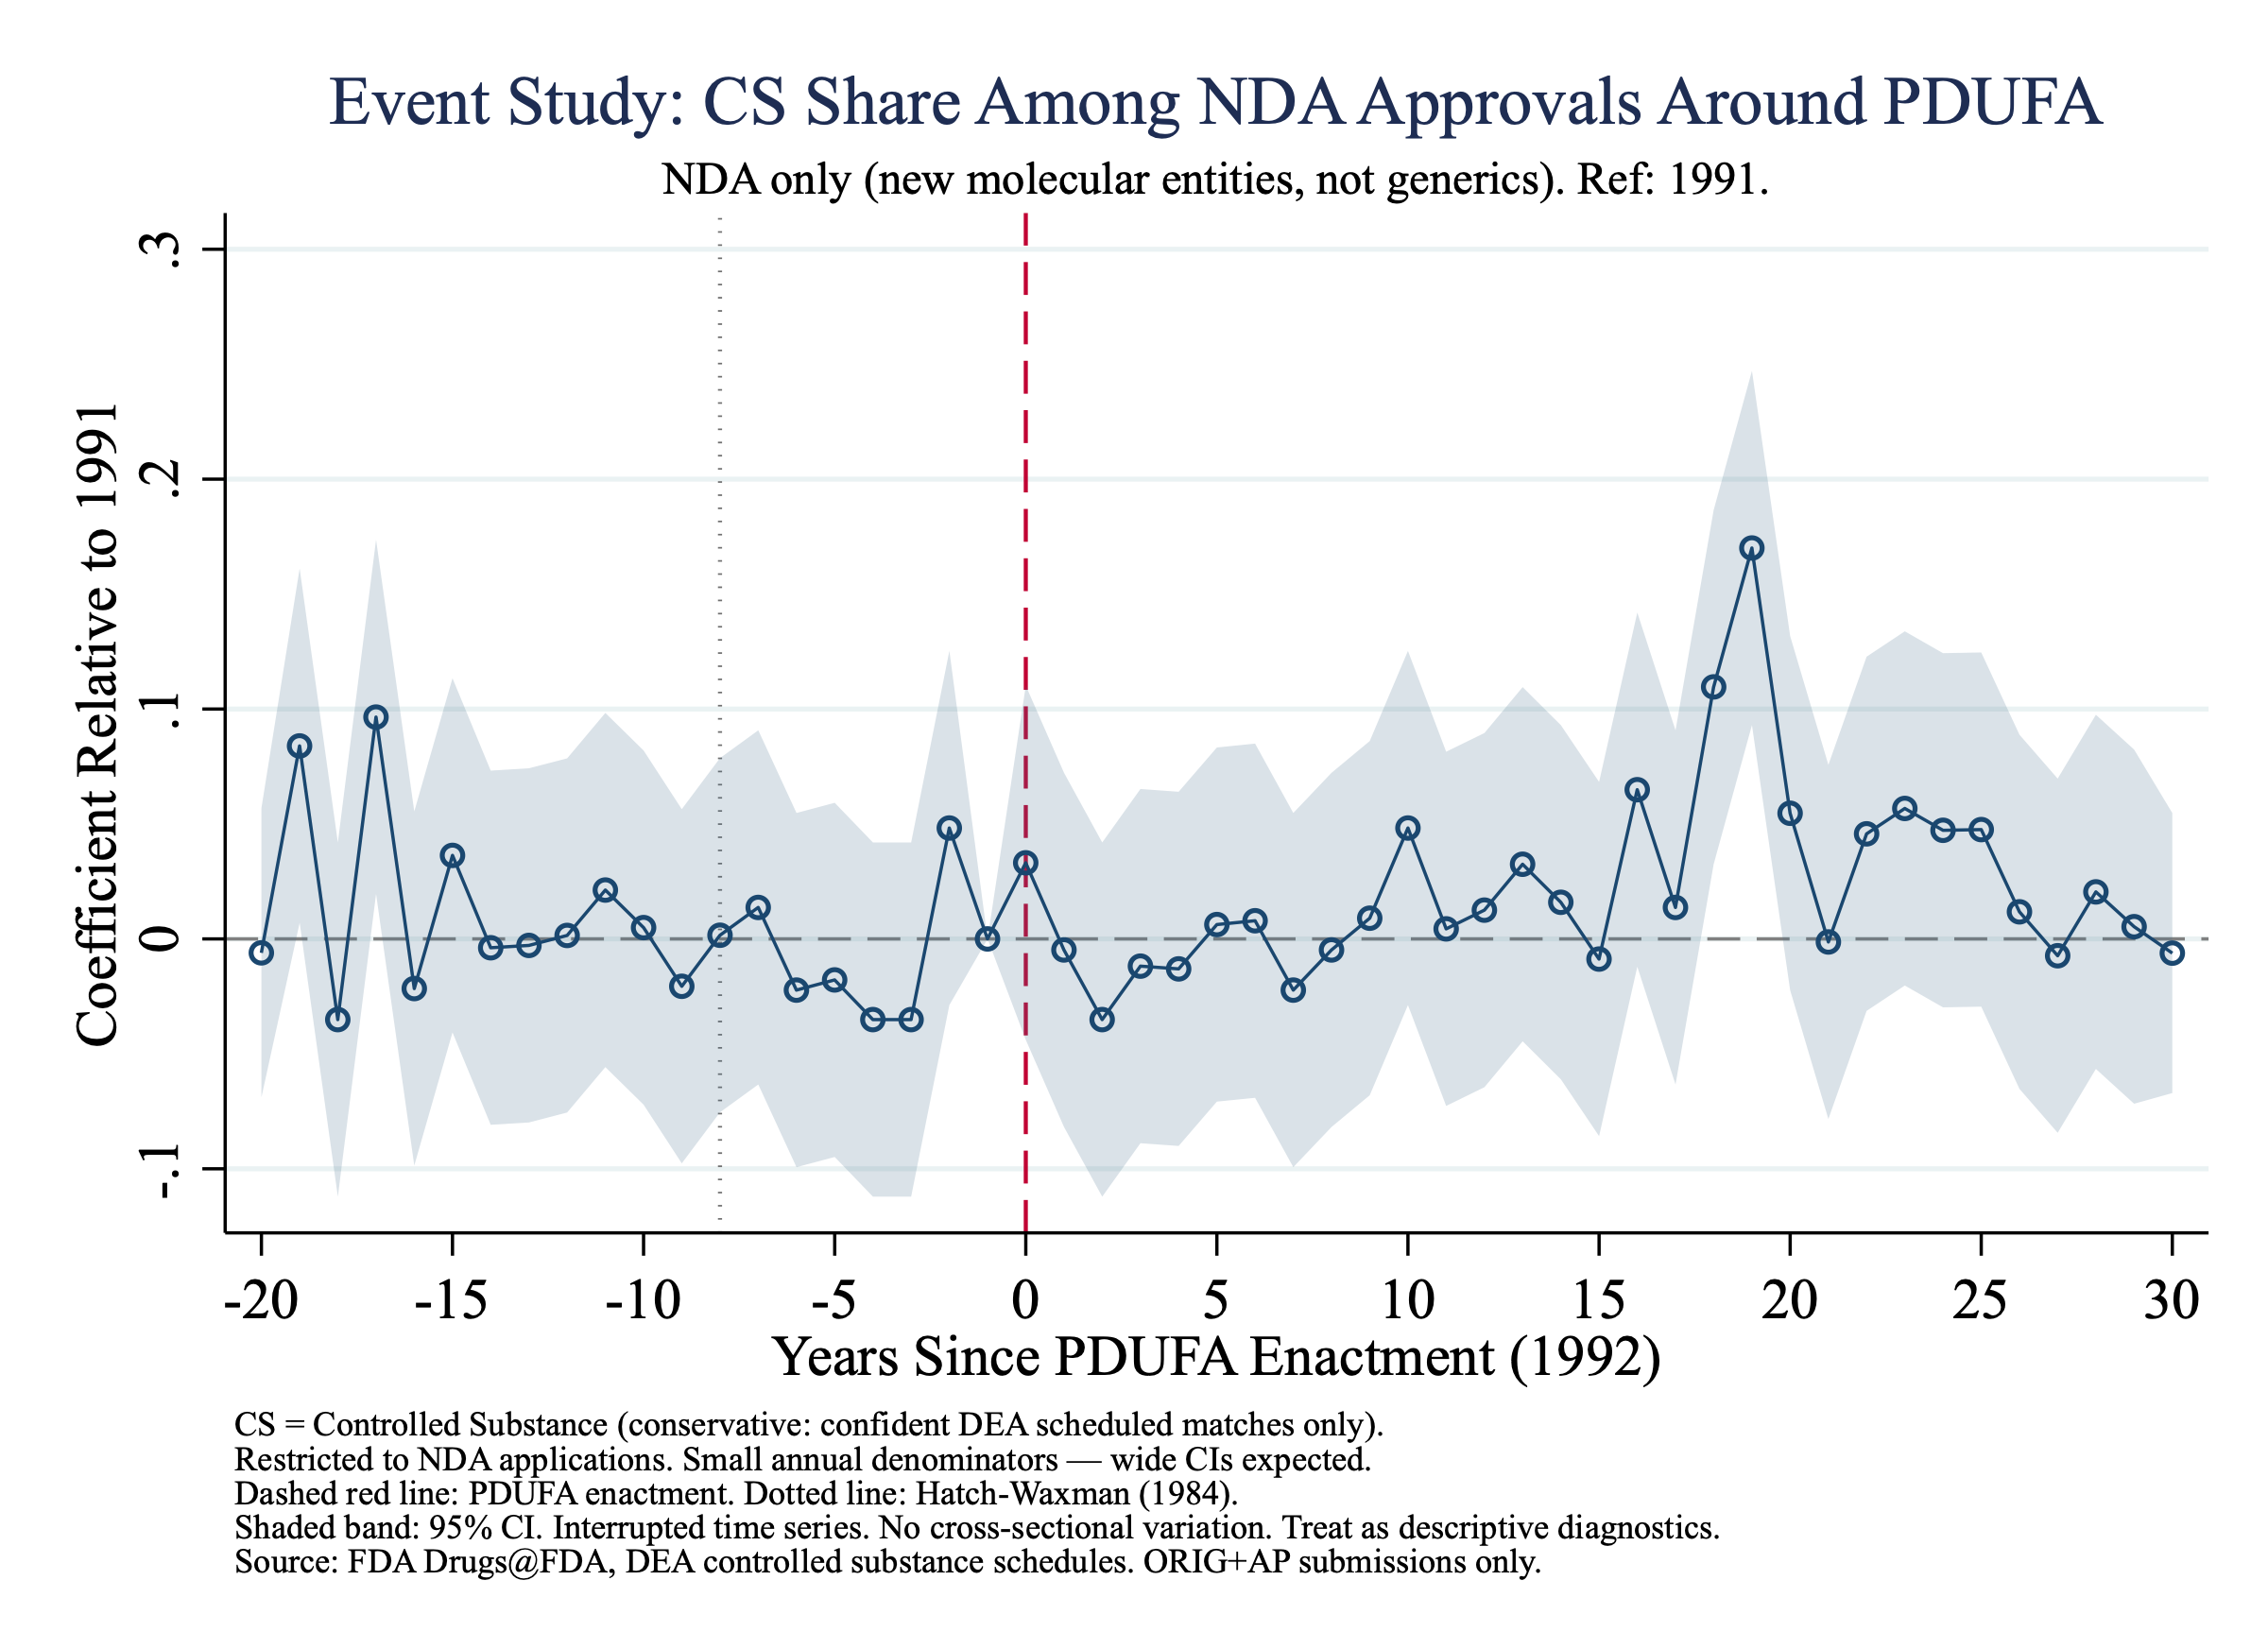
\includegraphics[width=0.92\textwidth]{../output/figures/stata/event_study_cs_share_nda.png}
\caption{PDUFA event study: NDA-only sample. CS share among new drug applications. Event time 0 = 1992. Reference: $\tau = -1$.}
\label{fig:event_study_nda}
\end{figure}

Figure~\ref{fig:nda_share_level} shows the NDA CS share level series with pre-PDUFA and post-PDUFA mean reference lines. The post-PDUFA mean is slightly higher than the pre-PDUFA mean, but the time-series visual makes clear that the difference is concentrated in the 2009--2013 window.

\begin{figure}[htbp]
\centering
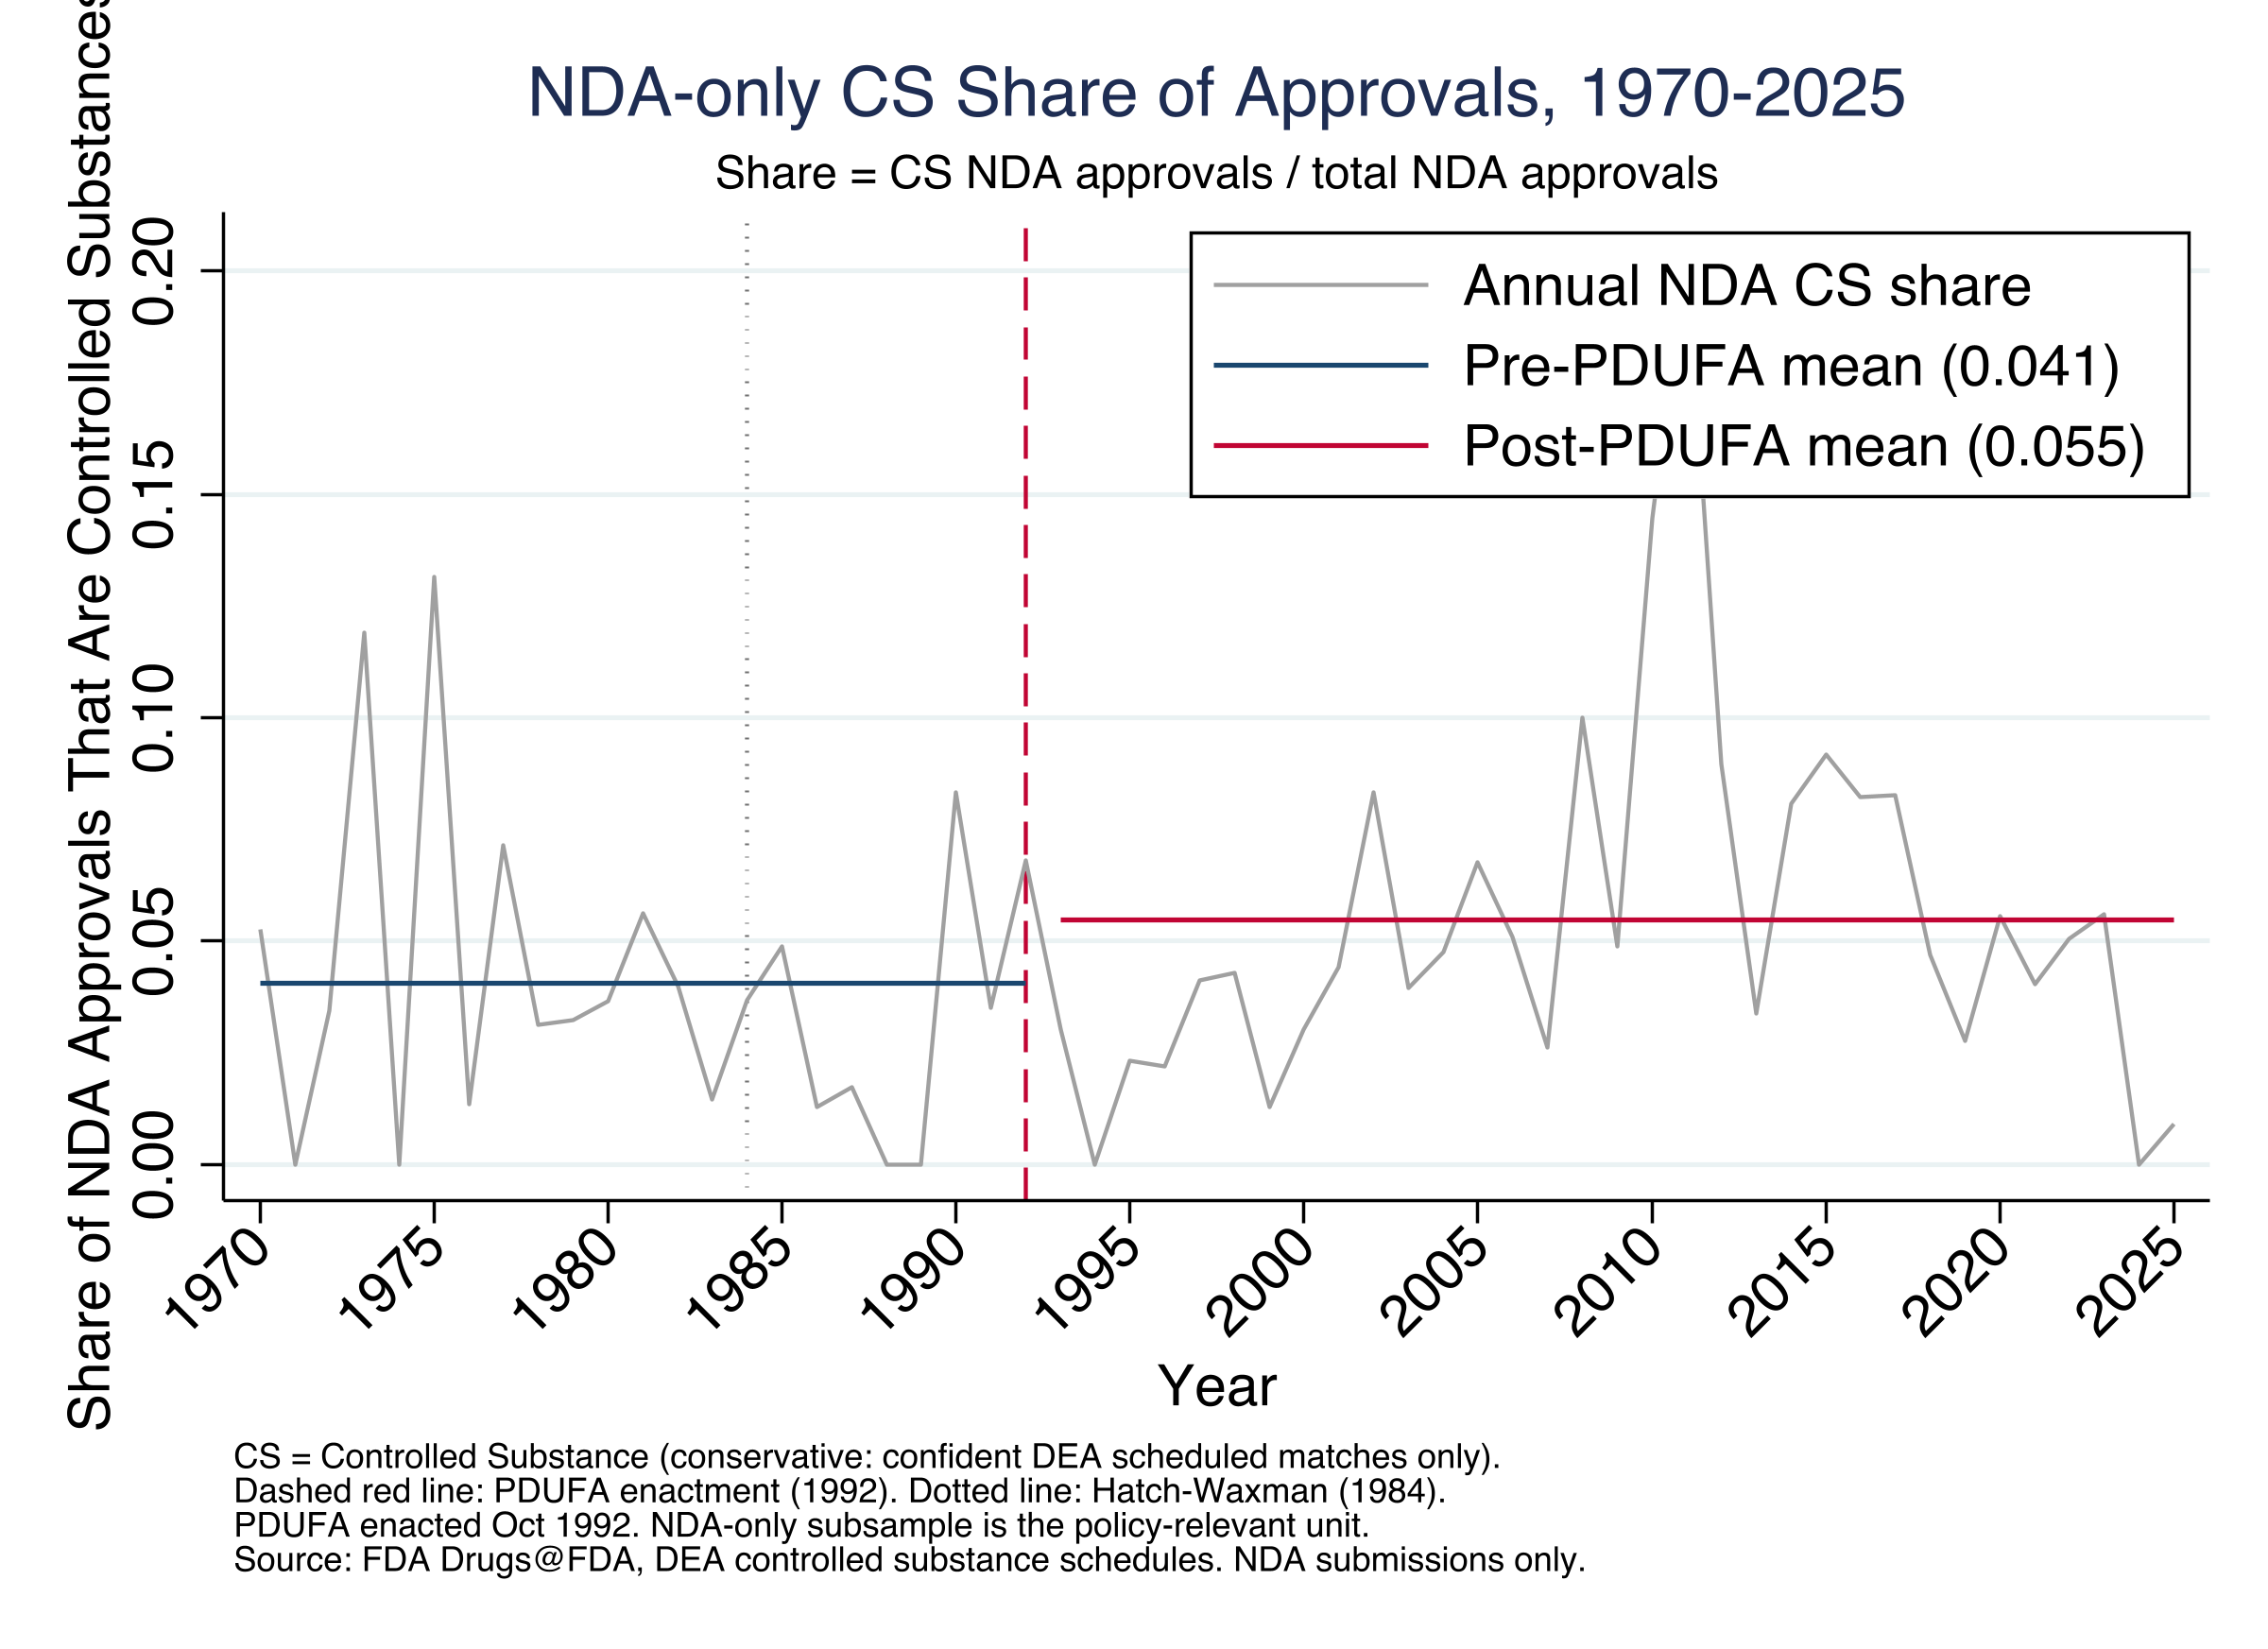
\includegraphics[width=0.92\textwidth]{../output/figures/stata/pdufa_nda_only_share.png}
\caption{NDA controlled-substance share, 1970--2025, with pre/post-PDUFA mean reference lines.}
\label{fig:nda_share_level}
\end{figure}

Table~\ref{tab:pdufa_poisson} reports Poisson rate models for the NDA CS count under three trend specifications. Column~(1) absorbs all year-level variation through year fixed effects. Column~(2) replaces year fixed effects with a single linear time trend. Column~(3) adds group-specific linear trends, allowing the CS and non-CS NDA streams to follow different secular paths. The post-PDUFA incidence-rate ratio in column~(1) is 1.46 ($p = 0.060$), consistent with a 46\% higher CS approval rate post-PDUFA after absorbing year-level variation. Under group-specific trends, the IRR is 1.19 with a 95\% confidence interval of $[0.59, 2.39]$, $p = 0.62$. The point estimate is essentially uninformative: it places the user-fee composition effect on the NDA margin in a band that includes a 41\% reduction and a 139\% increase, with mass concentrated around no effect. The fact that the apparent year-FE elevation is absorbed once group-specific trends accommodate the differential pre/post growth in CS and non-CS NDA streams is the central diagnostic of this section.

\begin{table}[htbp]
\centering
\begin{threeparttable}
\caption{PDUFA NDA-Only Poisson Rate Models: Sensitivity to Trend Controls}
\label{tab:pdufa_poisson}
\small
\begin{tabular}{lccc}
\toprule
 & (1) Year FE & (2) Linear trend & (3) Group trends \\
\midrule
IRR & 1.456 & 1.456 & 1.190 \\
$z$-statistic & 1.879 & 1.832 & 0.490 \\
$p$-value & 0.060 & 0.067 & 0.624 \\
95\% CI & [0.98, 2.16] & [0.97, 2.18] & [0.59, 2.39] \\
\midrule
Observations & \multicolumn{3}{c}{Annual, 1970--2025, NDA only} \\
Exposure & \multicolumn{3}{c}{Total NDA approvals} \\
\bottomrule
\end{tabular}
\begin{tablenotes}
\footnotesize
\item IRR = incidence-rate ratio for the $\text{post\_pdufa} \times \text{is\_cs}$ interaction. Robust standard errors.
\item Column (3) adds separate linear time trends for the CS and non-CS NDA series.
\end{tablenotes}
\end{threeparttable}
\end{table}

Figure~\ref{fig:nda_dd_event} reports the event-study DD coefficients from the NDA-only stacked Poisson specification. The IRR profile sits near unity for all pre-policy event times, consistent with parallel pre-trends. Post-policy IRRs drift upward gradually, peak around event times 17--19 (2009--2011), and subside thereafter. This pattern --- a late-rising post-policy departure that does not appear near the policy date --- is inconsistent with a PDUFA composition effect operating through review-time incentives and is instead consistent with a delayed industry product cycle, as Section~\ref{sec:results_spike} documents at the drug level.

\begin{figure}[htbp]
\centering
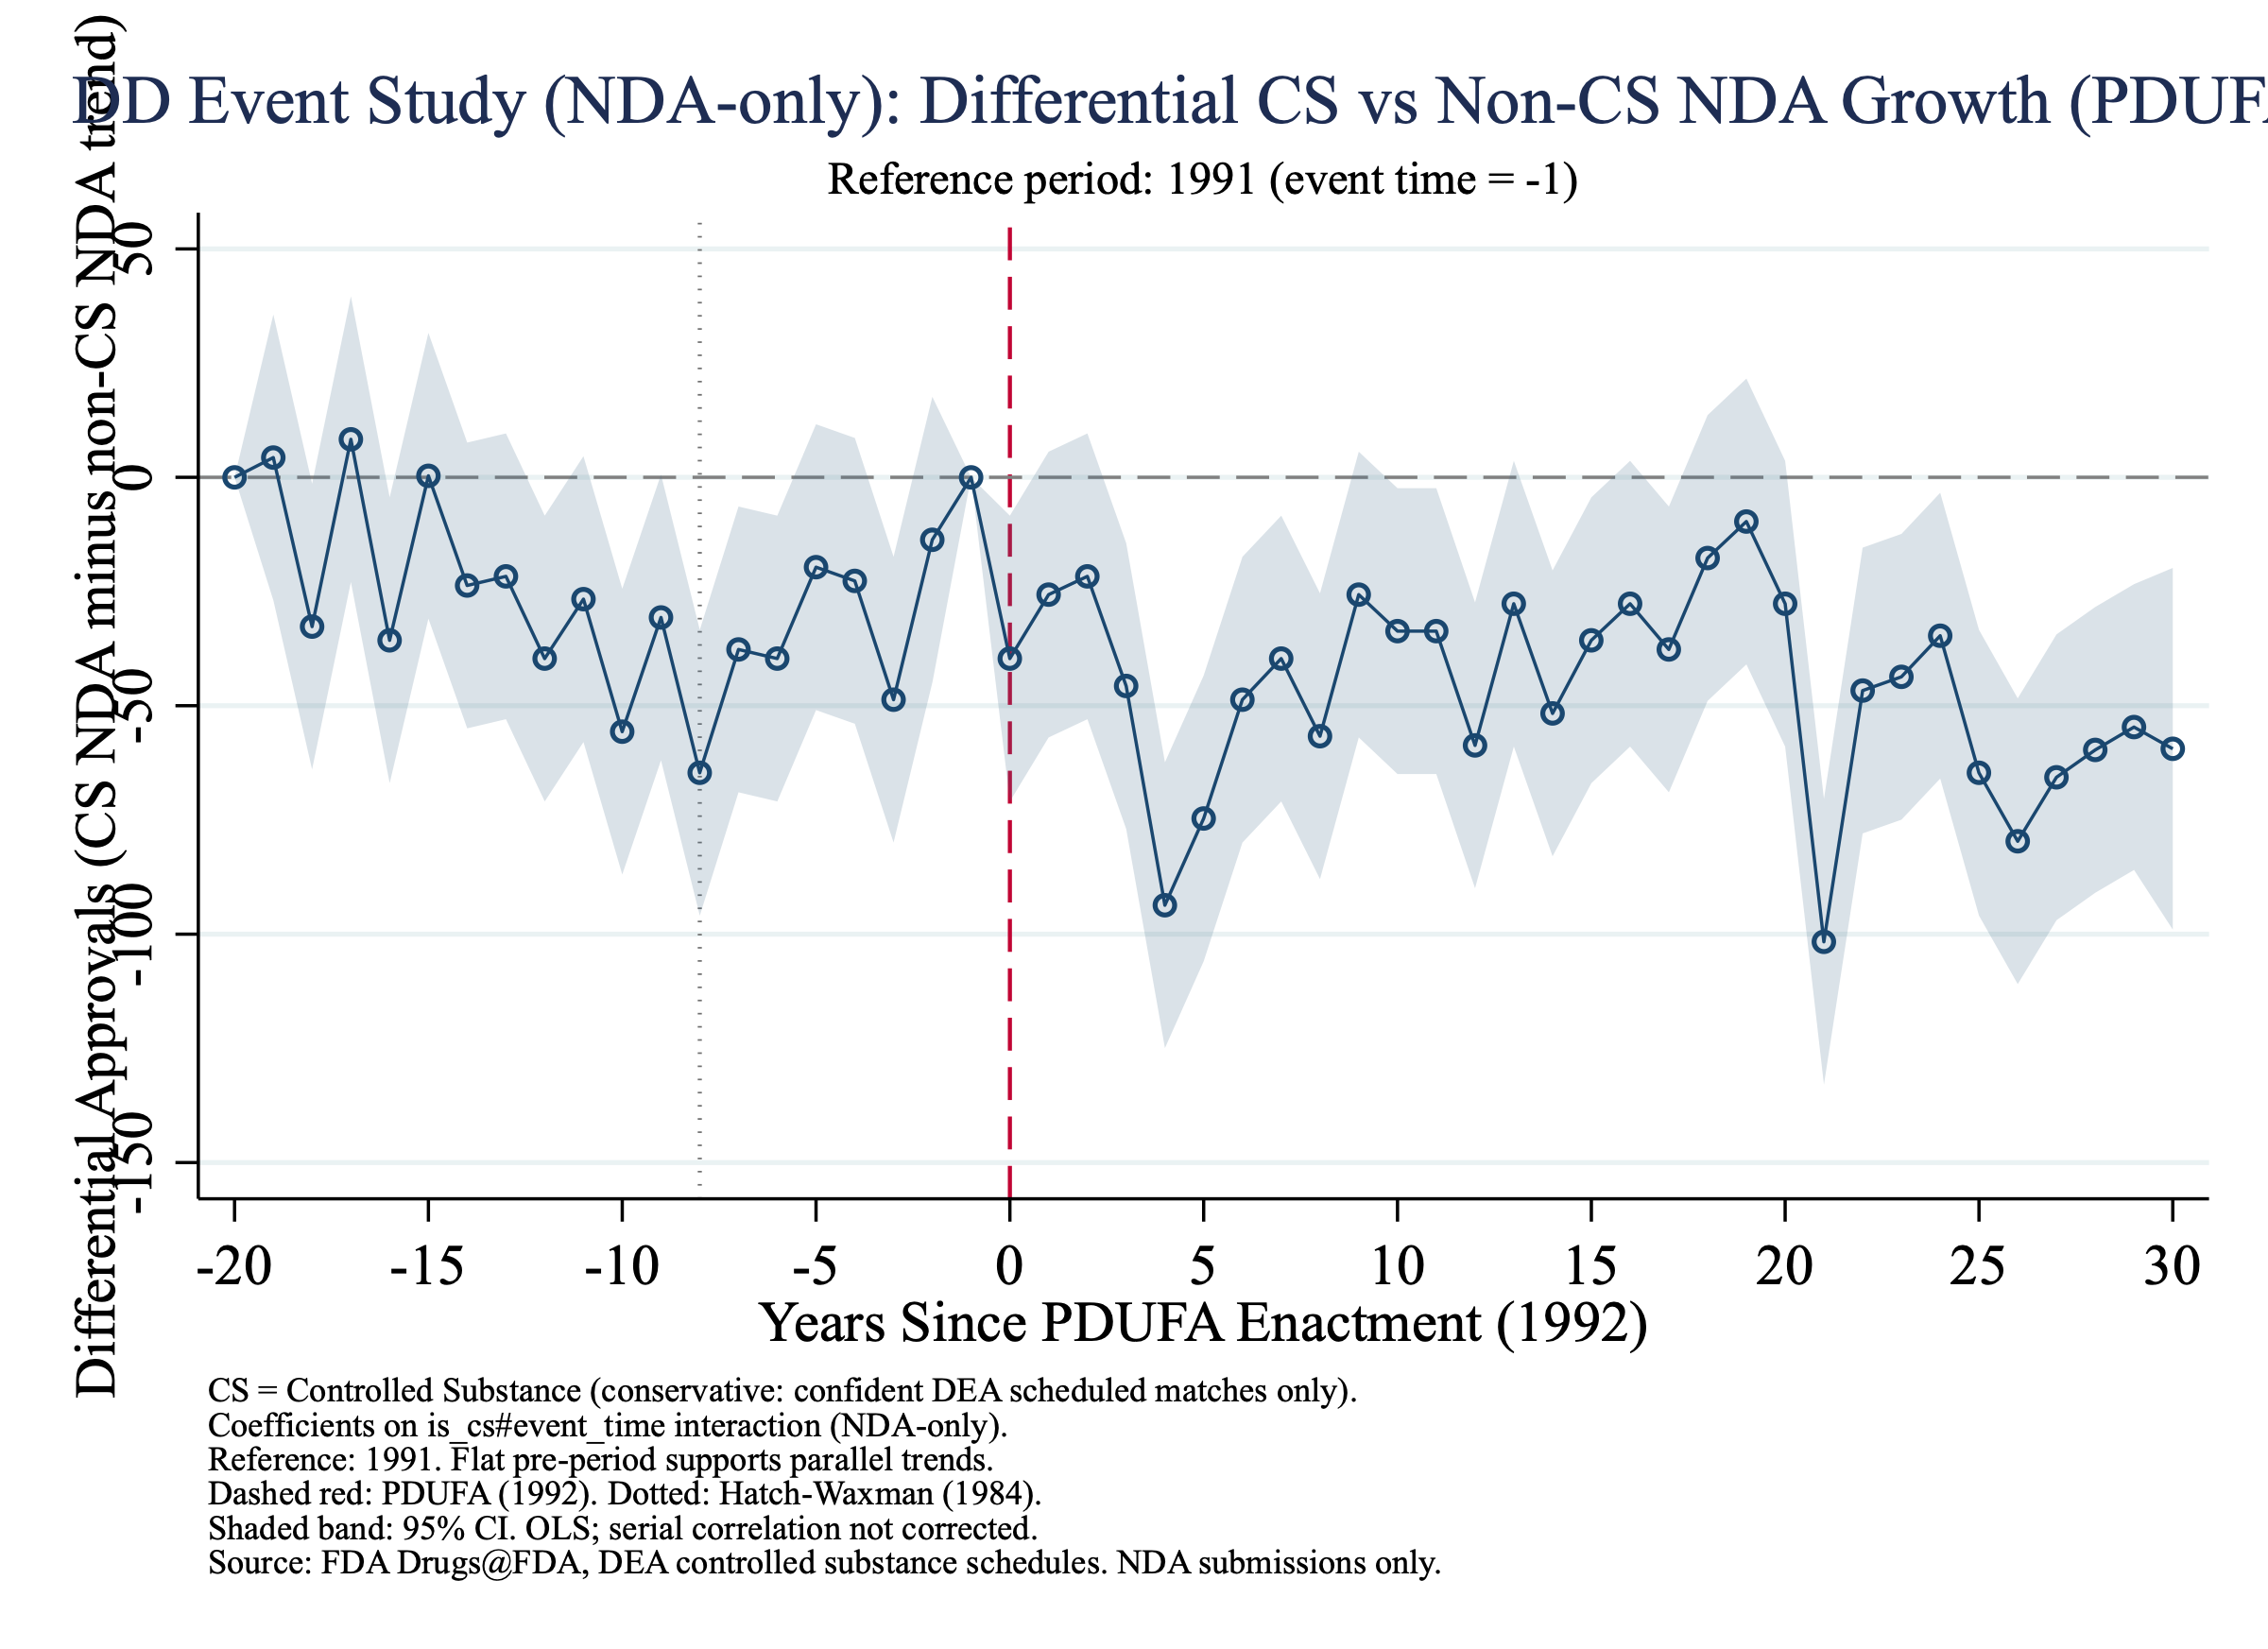
\includegraphics[width=0.92\textwidth]{../output/figures/stata/pdufa_nda_only_dd_event_study.png}
\caption{PDUFA NDA-only stacked Poisson DD event study. IRRs for $\text{CS} \times \mathbf{1}[\tau]$ interactions. Reference: $\tau = -1$ (1991). End-caps at $[-20, +30]$. 95\% CI.}
\label{fig:nda_dd_event}
\end{figure}

\subsection{Rate Versus Count Decomposition}

Figure~\ref{fig:nda_rate_count} decomposes the NDA result into a rate panel and a count panel. Panel~A shows the CS share of NDA approvals; Panel~B shows the absolute counts of CS and non-CS NDA approvals. The two panels are simultaneously consistent: the CS rate rises modestly after 1992 even as the absolute volume of non-CS NDA approvals grows faster in levels. Reading the rate alone could overstate any compositional shift; reading the count alone could understate it. Together they clarify that the apparent post-PDUFA NDA elevation reflects a small numerator increase concentrated in a narrow window, not a sustained reorientation of the NDA portfolio.

\begin{figure}[htbp]
\centering
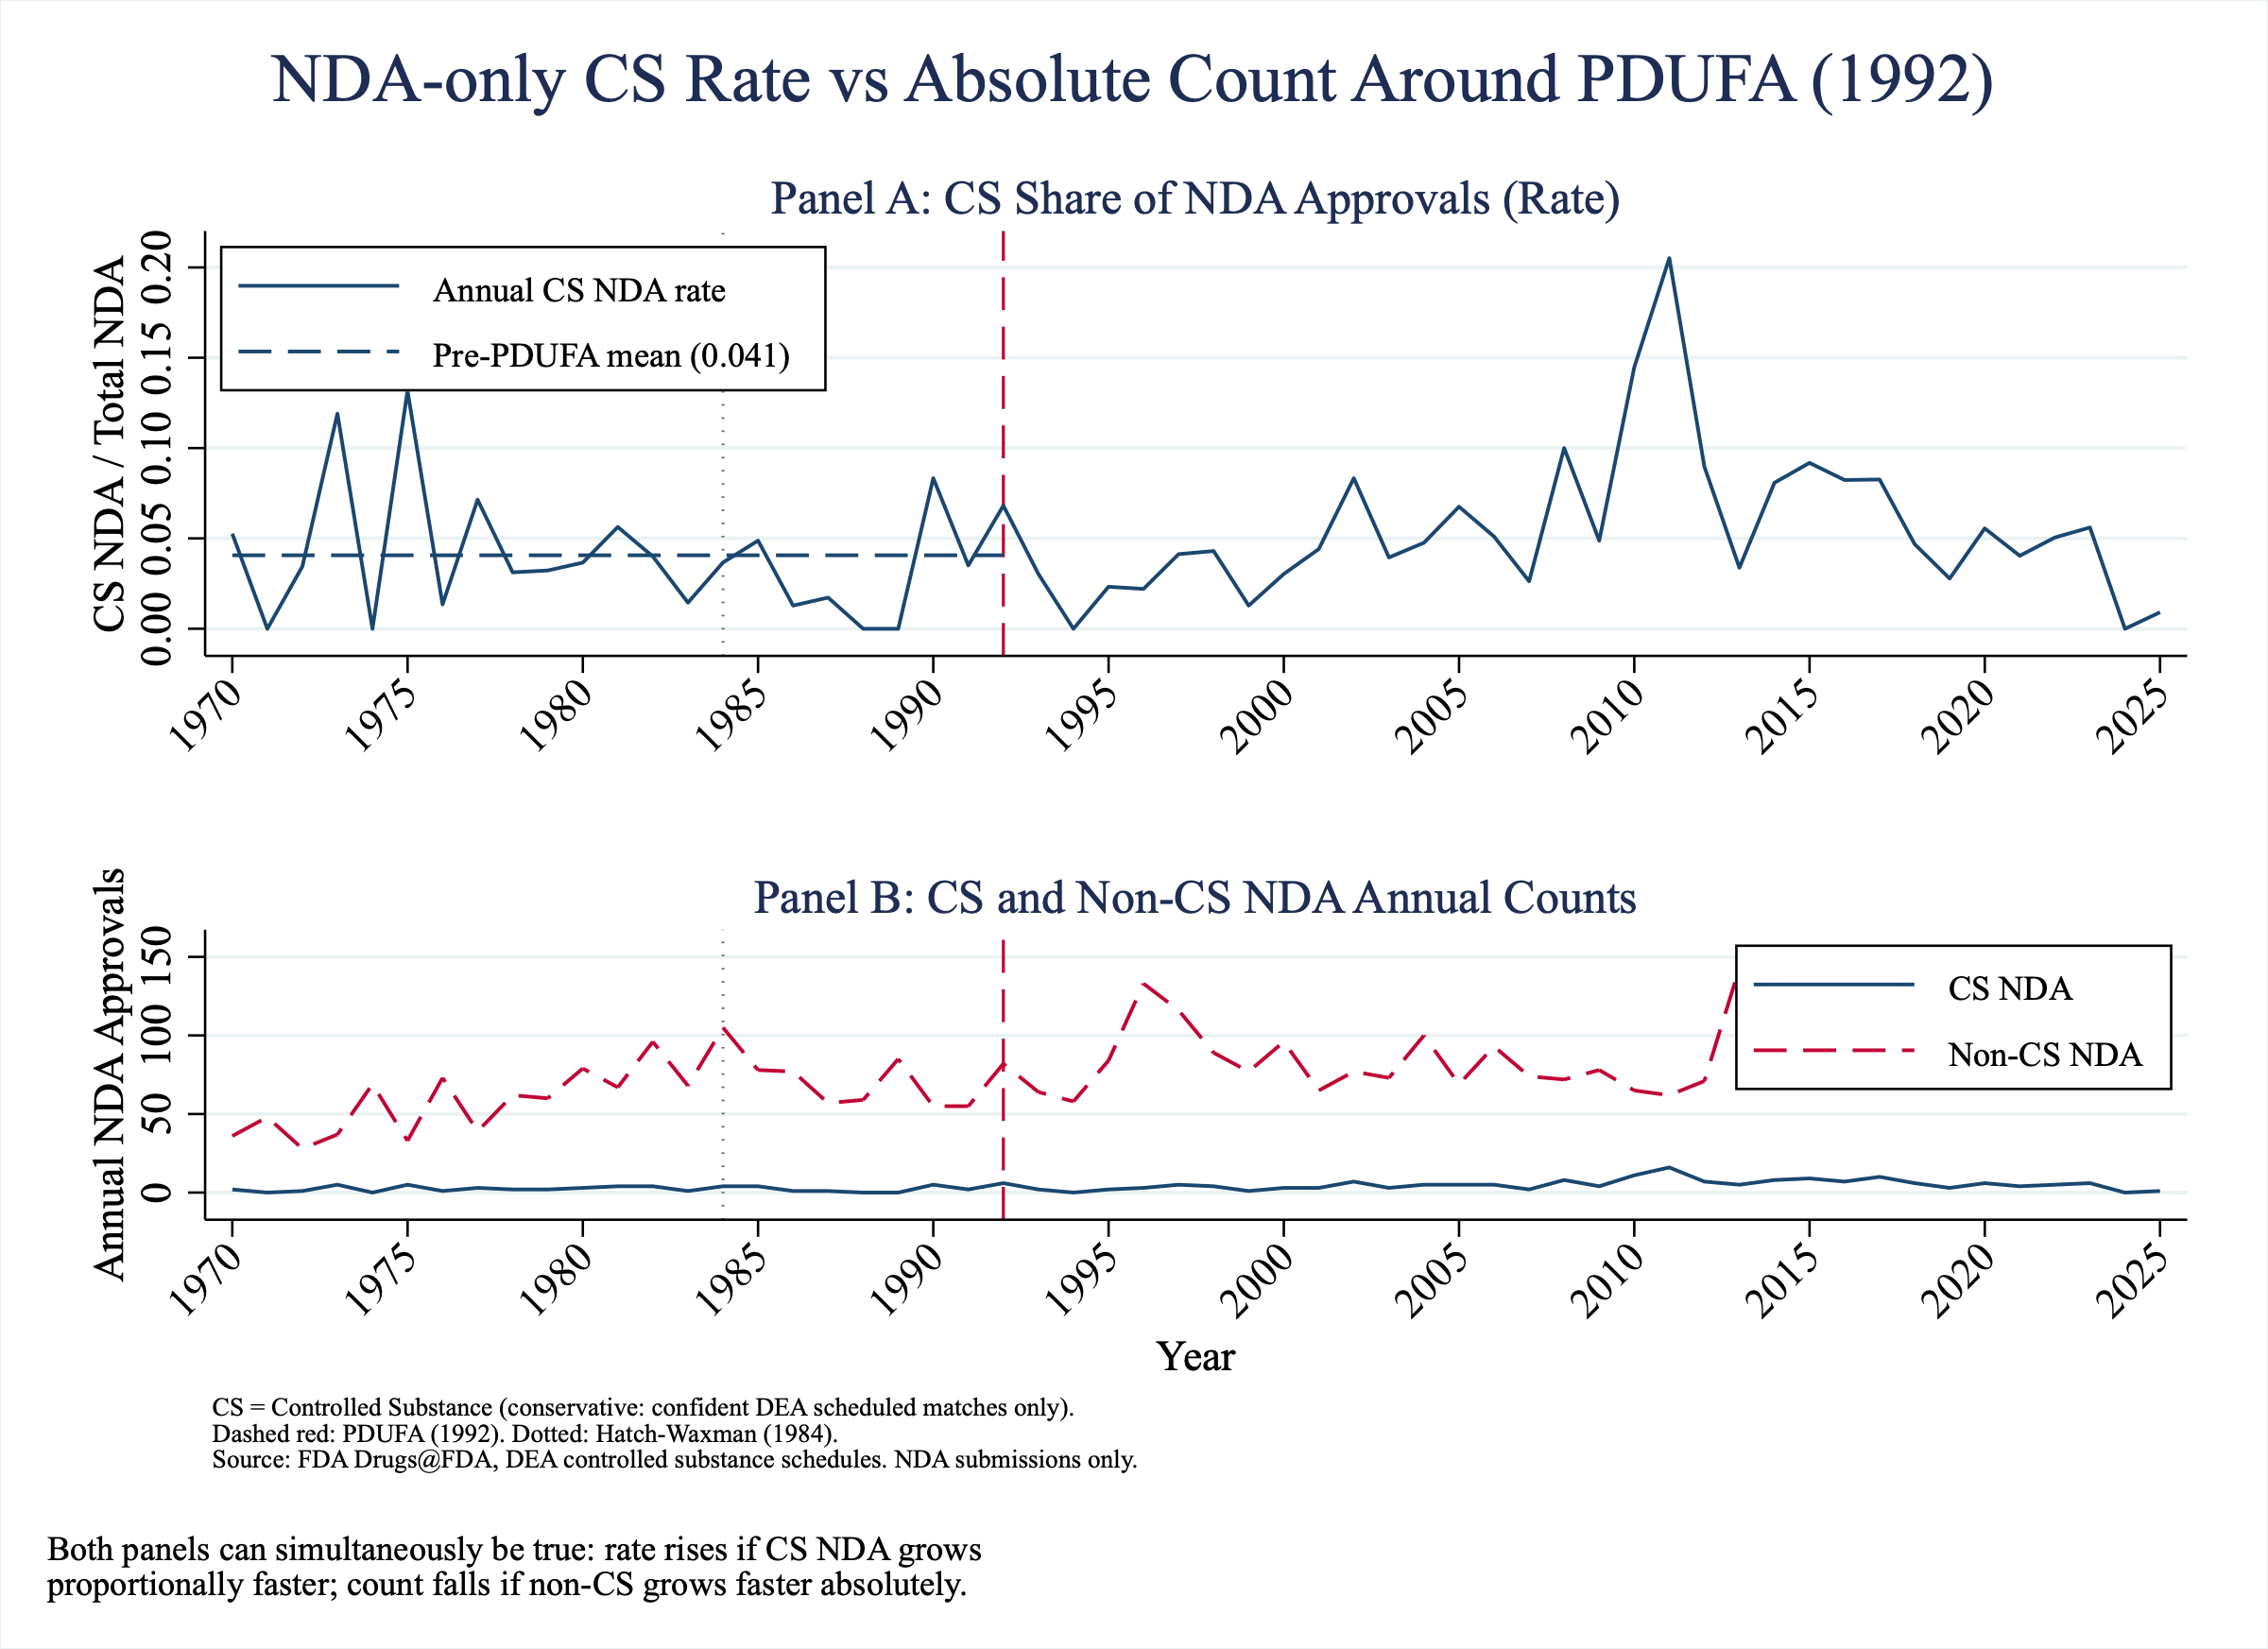
\includegraphics[width=0.92\textwidth]{../output/figures/stata/pdufa_nda_rate_vs_count.png}
\caption{NDA CS approvals: rate (Panel A) and absolute count (Panel B). Panel A shows CS share among NDA approvals with pre-PDUFA mean reference line. Panel B shows annual CS NDA count vs.\ non-CS NDA count.}
\label{fig:nda_rate_count}
\end{figure}

\subsection{The 2009--2013 CS NDA Spike}
\label{sec:results_spike}

The event-study and time-series evidence point to a cluster of Schedule~II NDA approvals concentrated in 2009--2013. Table~\ref{tab:spike_drugs} lists representative CS NDA approvals from this window, identifying the brand name, active ingredient, sponsor, and DEA schedule for each drug. Four features stand out. First, 43 CS NDAs were approved in this five-year window, compared with an average of roughly six to eight per year in the preceding decade. Second, 2011 alone accounts for 16 CS NDA approvals --- by far the largest single-year count in the sample. Third, 25 of the 43 approvals (58\%) are Schedule~II, the most restrictive category for drugs with accepted medical use. Fourth, the drug list maps closely onto the well-documented wave of branded extended-release and abuse-deterrent opioid formulations that characterized the late-2000s pharmaceutical market: the reformulated OxyContin (Purdue Pharma, 2010), Exalgo (Specgx, 2010), Embeda (Alpharma, 2009), Suboxone (Indivior, 2010), Zohydro ER (Zogenix, 2012), and related products.

\begin{table}[htbp]
\centering
\begin{threeparttable}
\caption{CS NDA Approvals, 2009--2013 (Selected)}
\label{tab:spike_drugs}
\small
\begin{tabular}{llllr}
\toprule
Year & Brand Name & Active Ingredient & Sponsor & Sched. \\
\midrule
2009 & ONSOLIS & Fentanyl citrate & ADALVO & II \\
2009 & EMBEDA & Morphine sulfate; naltrexone & ALPHARMA & II \\
2009 & CODEINE SULFATE & Codeine sulfate & HIKMA & II \\
2009 & EDLUAR & Zolpidem tartrate & VIATRIS & IV \\
2010 & EXALGO & Hydromorphone HCl & SPECGX LLC & II \\
2010 & OXYCONTIN & Oxycodone HCl & PURDUE PHARMA & II \\
2010 & SUBOXONE & Buprenorphine; naloxone & INDIVIOR & III \\
2010 & BUTRANS & Buprenorphine & PURDUE PHARMA & III \\
2010 & AXIRON & Testosterone & ELI LILLY & III \\
2010 & LYRICA & Pregabalin & UPJOHN & V \\
2011 & ANDROGEL & Testosterone & BESINS HLTHCARE & III \\
2011 & INTERMEZZO & Zolpidem tartrate & PURDUE PHARMA & IV \\
2012 & ZOHYDRO ER & Hydrocodone bitartrate & ZOGENIX & II \\
\midrule
\multicolumn{5}{l}{\textit{Full 2009--2013 window: 43 CS NDAs; 25 Schedule~II (58\%); 2011 peak: 16 approvals.}} \\
\bottomrule
\end{tabular}
\begin{tablenotes}
\footnotesize
\item Selected rows for illustration. Full list in \texttt{output/tables/stata/cs\_nda\_2009\_2013\_drugs.csv}.
\item OxyContin (2010) is the reformulated abuse-deterrent NDA (NDA 022272), not the original 1995 approval.
\end{tablenotes}
\end{threeparttable}
\end{table}

The timing of these approvals --- seventeen to twenty-one years after PDUFA enactment --- and their close correspondence to a documented pharmaceutical product cycle make them difficult to attribute to user-fee incentives. Once the late-2000s opioid wave is allowed to load onto its own group-specific trend in column~(3) of Table~\ref{tab:pdufa_poisson}, the post-PDUFA IRR moves toward unity and the wide confidence interval $[0.59, 2.39]$ obtains.

\subsection{GDUFA Event Study: ANDA-Only}
\label{sec:results_gdufa}

Figure~\ref{fig:gdufa_event} reports the GDUFA event-study DD for the ANDA-only sample. Pre-policy event-time coefficients sit near zero, supporting the parallel-trends assumption over the 2002--2012 pre-GDUFA window. Post-policy IRRs decline through the 2015--2025 performance-goal era. The stacked Poisson DD specification (Table~\ref{tab:gdufa_results}) yields a year-FE IRR of $0.668$ ($p < 0.001$, 95\% CI $[0.55, 0.81]$), implying that the CS share of ANDA approvals fell by approximately one-third relative to the non-CS share after 2015. The level result is robust to a single linear time trend ($p = 0.008$).

\begin{figure}[htbp]
\centering
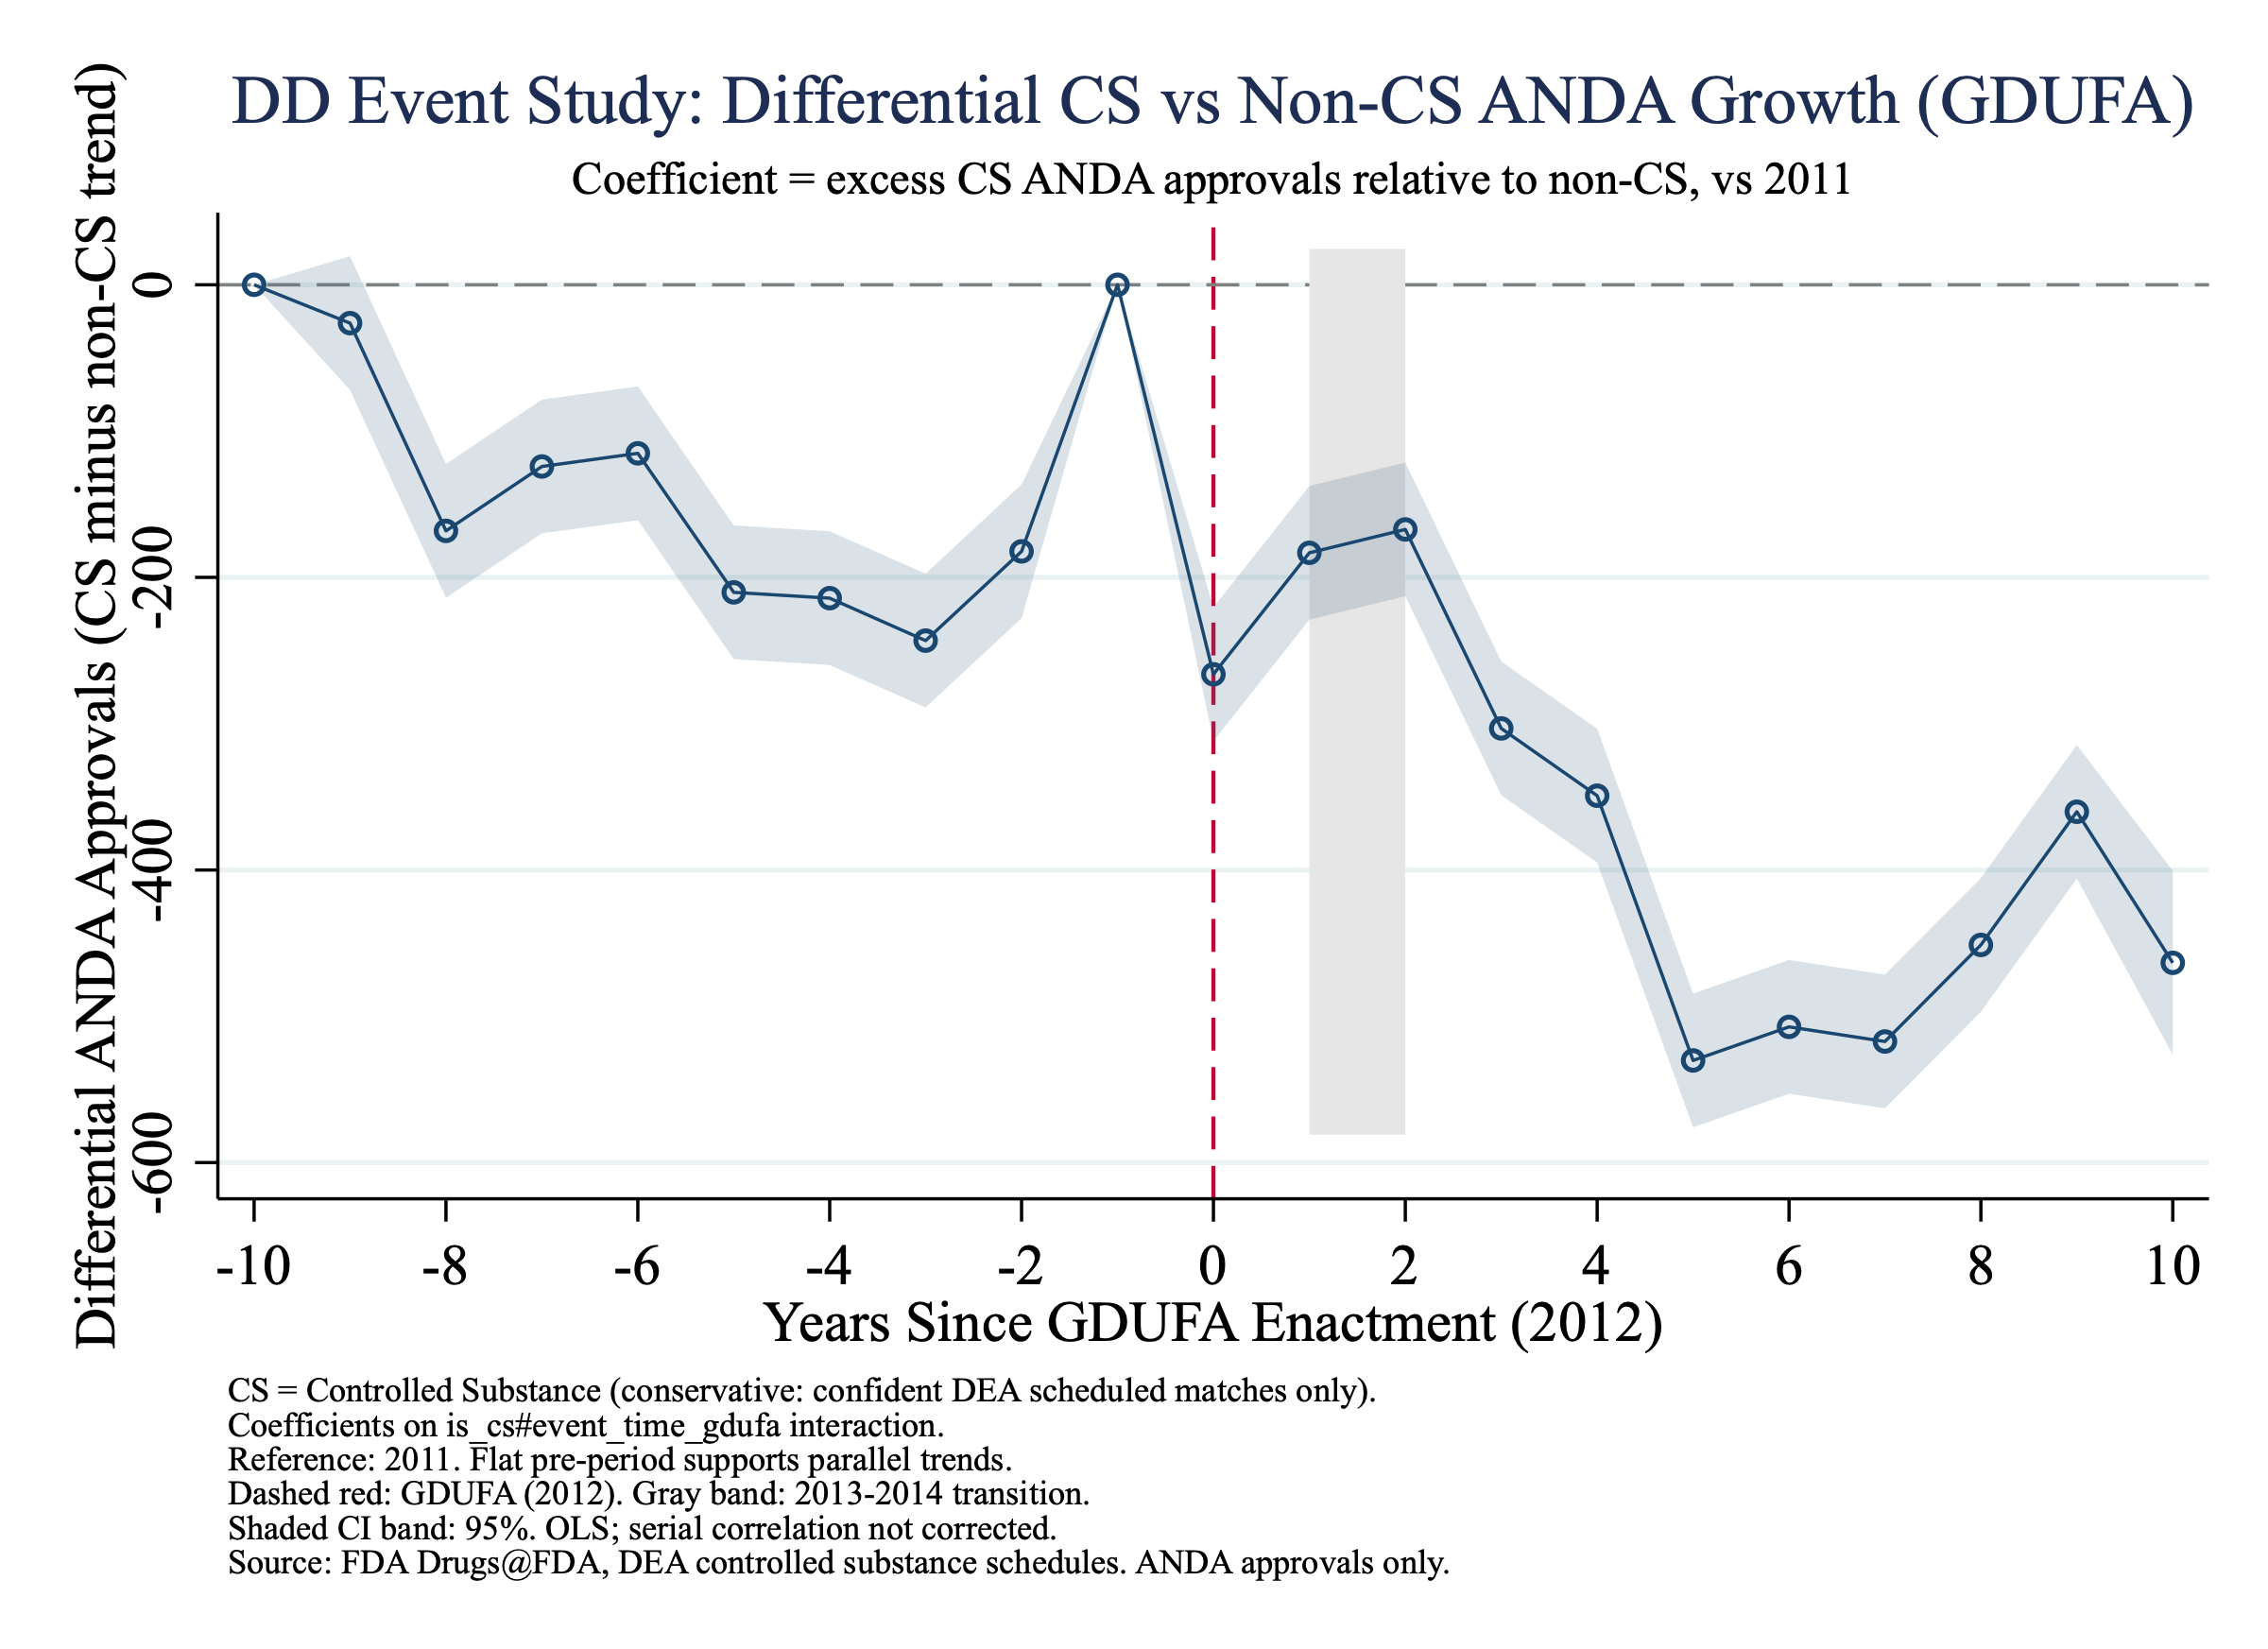
\includegraphics[width=0.92\textwidth]{../output/figures/stata/gdufa_dd_event_study.png}
\caption{GDUFA ANDA-only stacked Poisson DD event study. IRRs for $\text{CS} \times \mathbf{1}[\tau]$ interactions. Reference: $\tau = -1$ (2011). End-caps at $[-10, +10]$. Transition years 2013--2014 excluded. 95\% CI.}
\label{fig:gdufa_event}
\end{figure}

The robustness story changes once group-specific linear trends are added. Allowing the CS-ANDA and non-CS-ANDA series to follow their own pre-period trajectories yields an IRR of $1.38$ with a 95\% confidence interval of $[0.86, 2.21]$ and $p = 0.18$ --- a point estimate that not only fails to attain conventional significance but also flips sign relative to the year-FE specification. The level decline observed in the year-FE specification is absorbed once the analysis allows for the steady pre-policy decline in the CS share of ANDA approvals that began well before GDUFA. Read together, these results argue for the same null interpretation as the PDUFA evidence: the user-fee composition effect on the ANDA controlled-substance margin is not separately identified from a longer-running secular trend.

Figure~\ref{fig:gdufa_rate_count} decomposes the GDUFA result into rate (Panel A) and count (Panel B). Panel A shows the ANDA CS share declining from a pre-GDUFA mean of 10.8\% to a post-GDUFA mean of approximately 7.1\%. Panel B shows that both the CS ANDA count and the non-CS ANDA count declined in absolute terms after GDUFA, with the CS count falling proportionally more steeply. The decomposition makes clear that the year-FE result is a relative one --- both series fall, and the CS series falls faster --- which is consistent with the pre-existing trend interpretation rather than with a post-GDUFA structural break.

\begin{figure}[htbp]
\centering
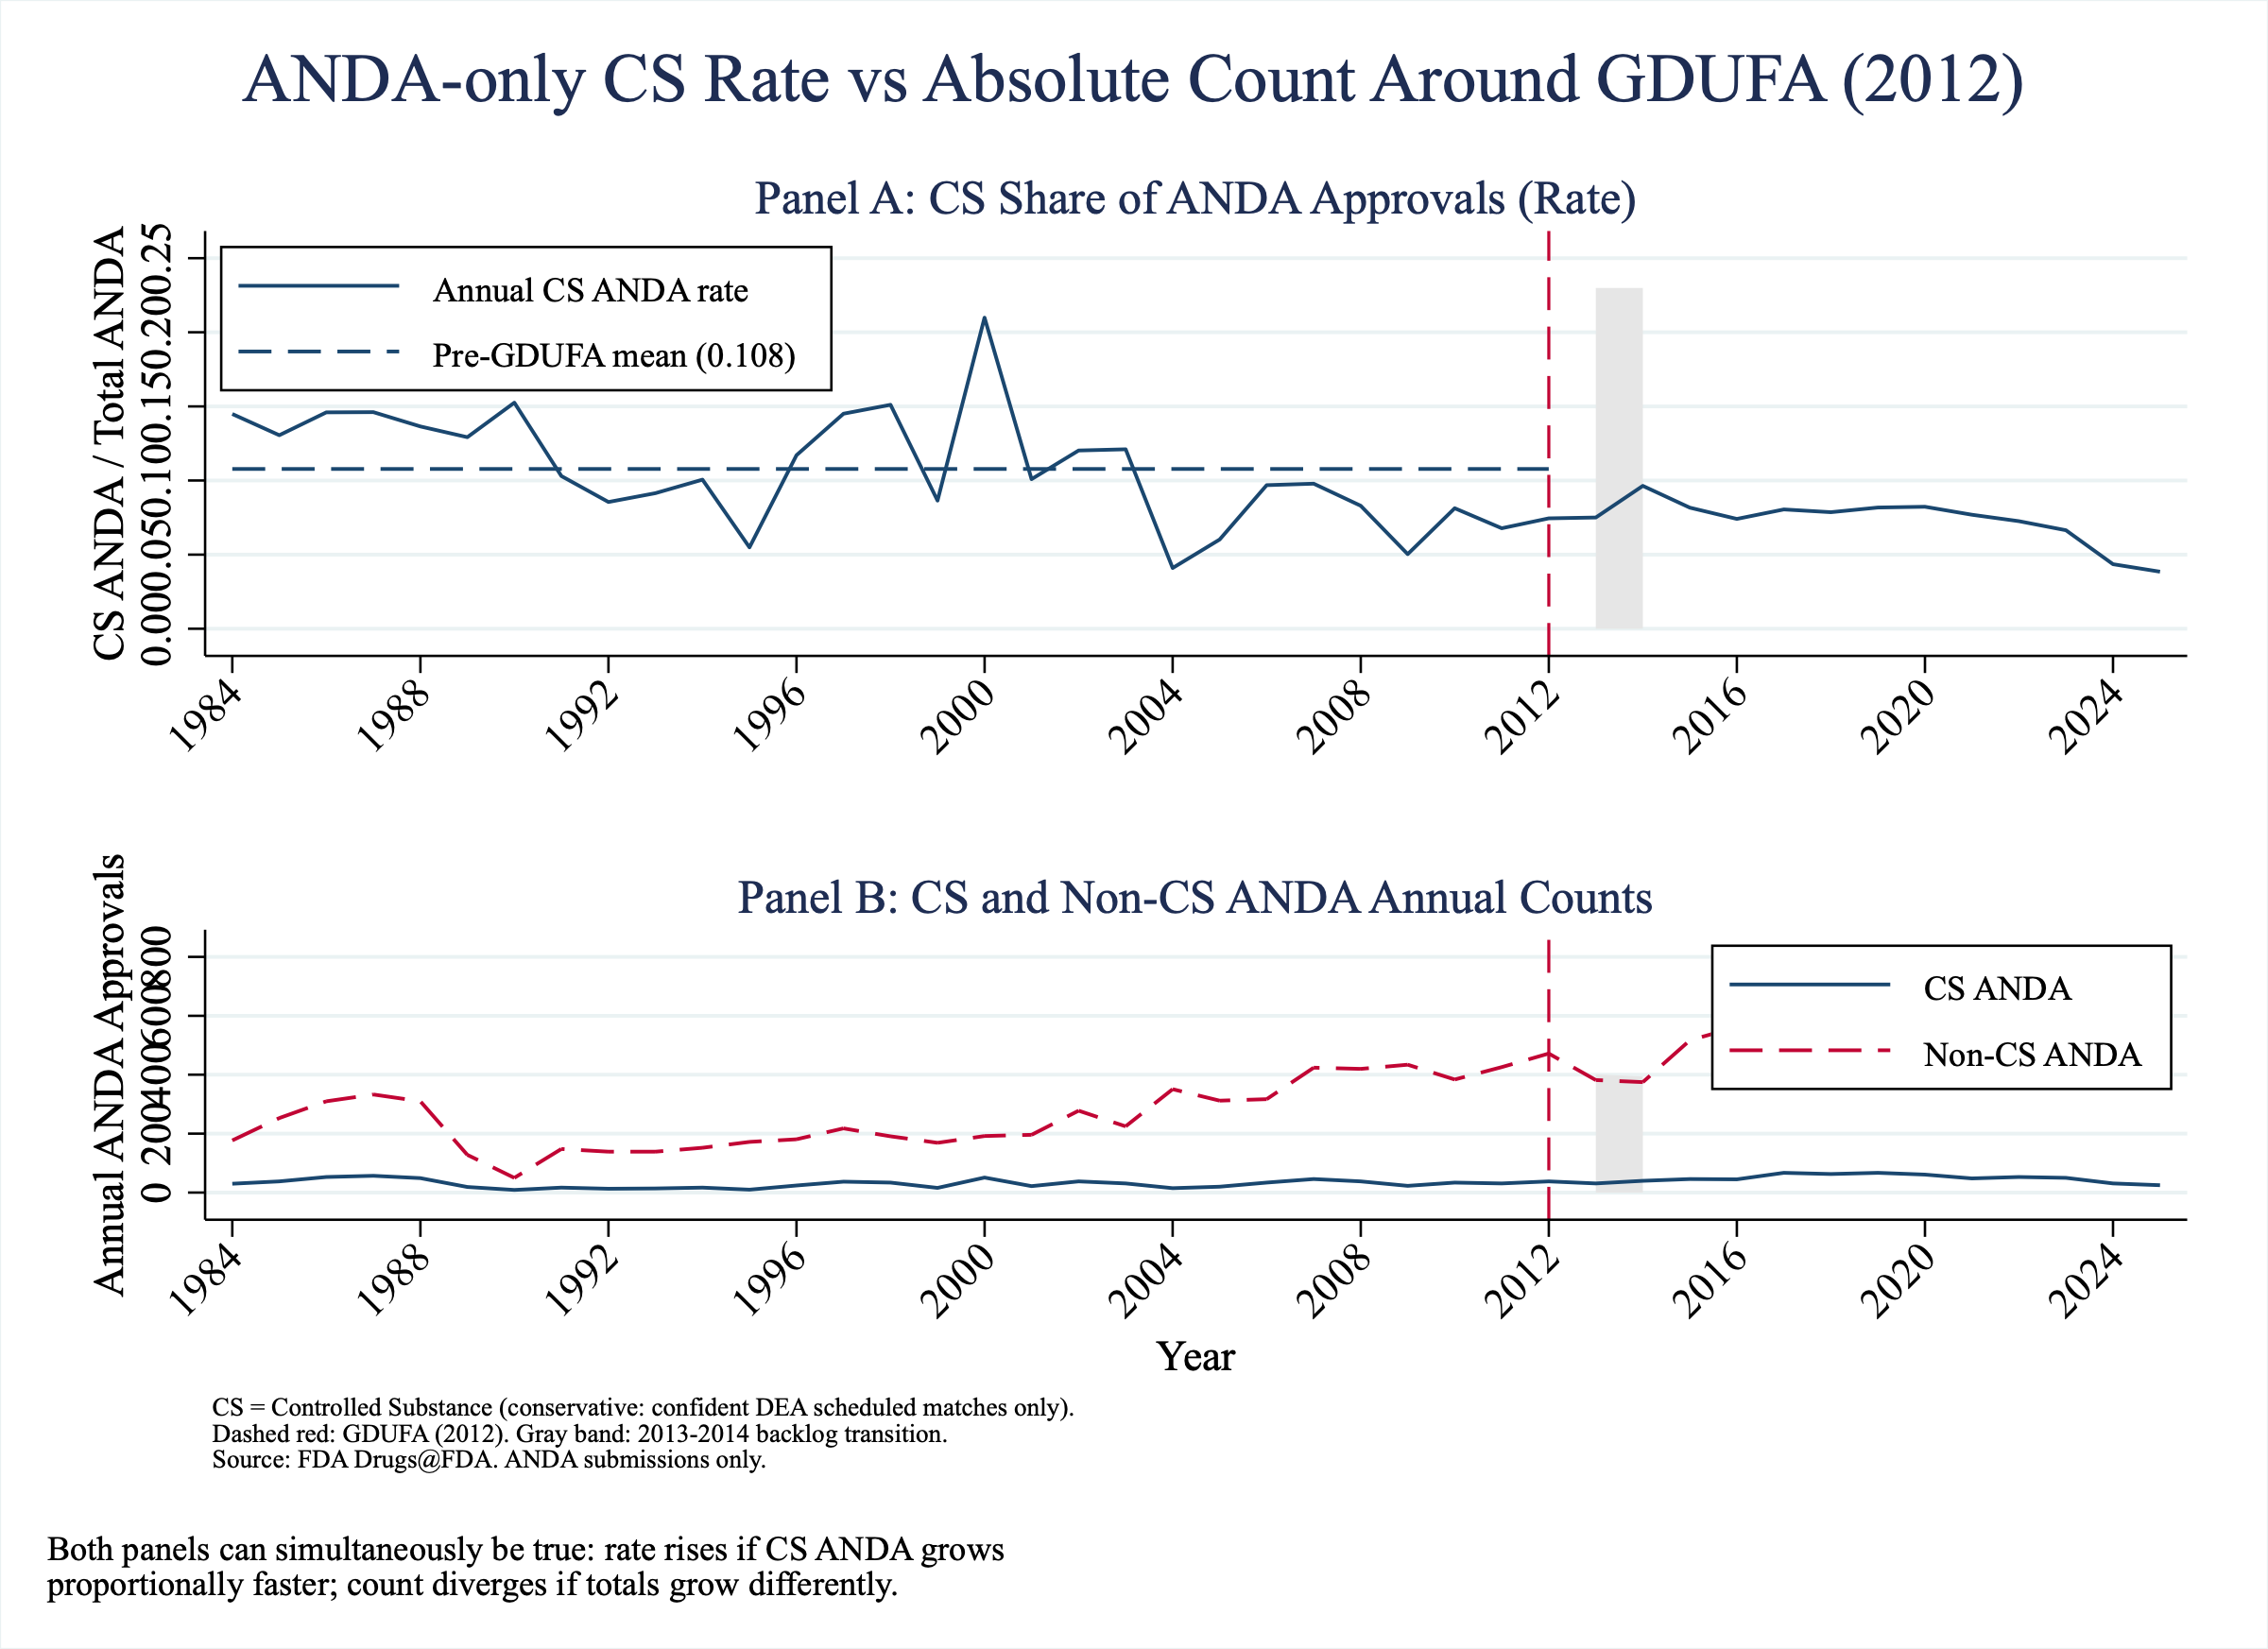
\includegraphics[width=0.92\textwidth]{../output/figures/stata/gdufa_anda_rate_vs_count.png}
\caption{GDUFA ANDA CS approvals: rate (Panel A) and absolute count (Panel B). Shaded region: 2013--2014 transition period.}
\label{fig:gdufa_rate_count}
\end{figure}

\begin{table}[htbp]
\centering
\begin{threeparttable}
\caption{GDUFA and PDUFA Stacked Poisson DD: Sensitivity to Trend Controls}
\label{tab:gdufa_results}
\small
\begin{tabular}{lcccc}
\toprule
 & Coef. & SE & IRR & 95\% CI \\
\midrule
\multicolumn{5}{l}{\textit{Panel A: GDUFA, ANDA-only}} \\
Year FE & $-0.403$ & $0.095$ & $0.668$ & $[0.55,\,0.81]$ \\
Linear trend & $-0.403$ & $0.152$ & $0.668$ & $[0.50,\,0.90]$ \\
Group-specific trends & $\phantom{-}0.323$ & $0.240$ & $1.382$ & $[0.86,\,2.21]$ \\
\midrule
\multicolumn{5}{l}{\textit{Panel B: PDUFA, NDA-only}} \\
Year FE & $\phantom{-}0.376$ & $0.200$ & $1.456$ & $[0.98,\,2.16]$ \\
Linear trend & $\phantom{-}0.376$ & $0.205$ & $1.456$ & $[0.97,\,2.18]$ \\
Group-specific trends & $\phantom{-}0.174$ & $0.356$ & $1.190$ & $[0.59,\,2.39]$ \\
\bottomrule
\end{tabular}
\begin{tablenotes}
\footnotesize
\item Stacked Poisson DD with log-total-approval exposure. Robust standard errors.
\item GDUFA excludes 2013--2014 transition years. PDUFA uses NDA-only sample.
\end{tablenotes}
\end{threeparttable}
\end{table}

\subsection{Sponsor Concentration}

Figure~\ref{fig:nda_hhi} and Figure~\ref{fig:gdufa_hhi} report Herfindahl--Hirschman Indices of sponsor concentration among CS NDA approvals (Figure~\ref{fig:nda_hhi}) and all ANDA approvals (Figure~\ref{fig:gdufa_hhi}). The CS NDA HHI is notably higher and more variable than the ANDA HHI, reflecting the smaller annual count of CS NDA approvals and the dominance of a small number of branded sponsors in certain years. The GDUFA era is associated with a visible decline in ANDA CS HHI, consistent with both the entry of additional generic sponsors and the decline in CS ANDA volume.

\begin{figure}[htbp]
\centering
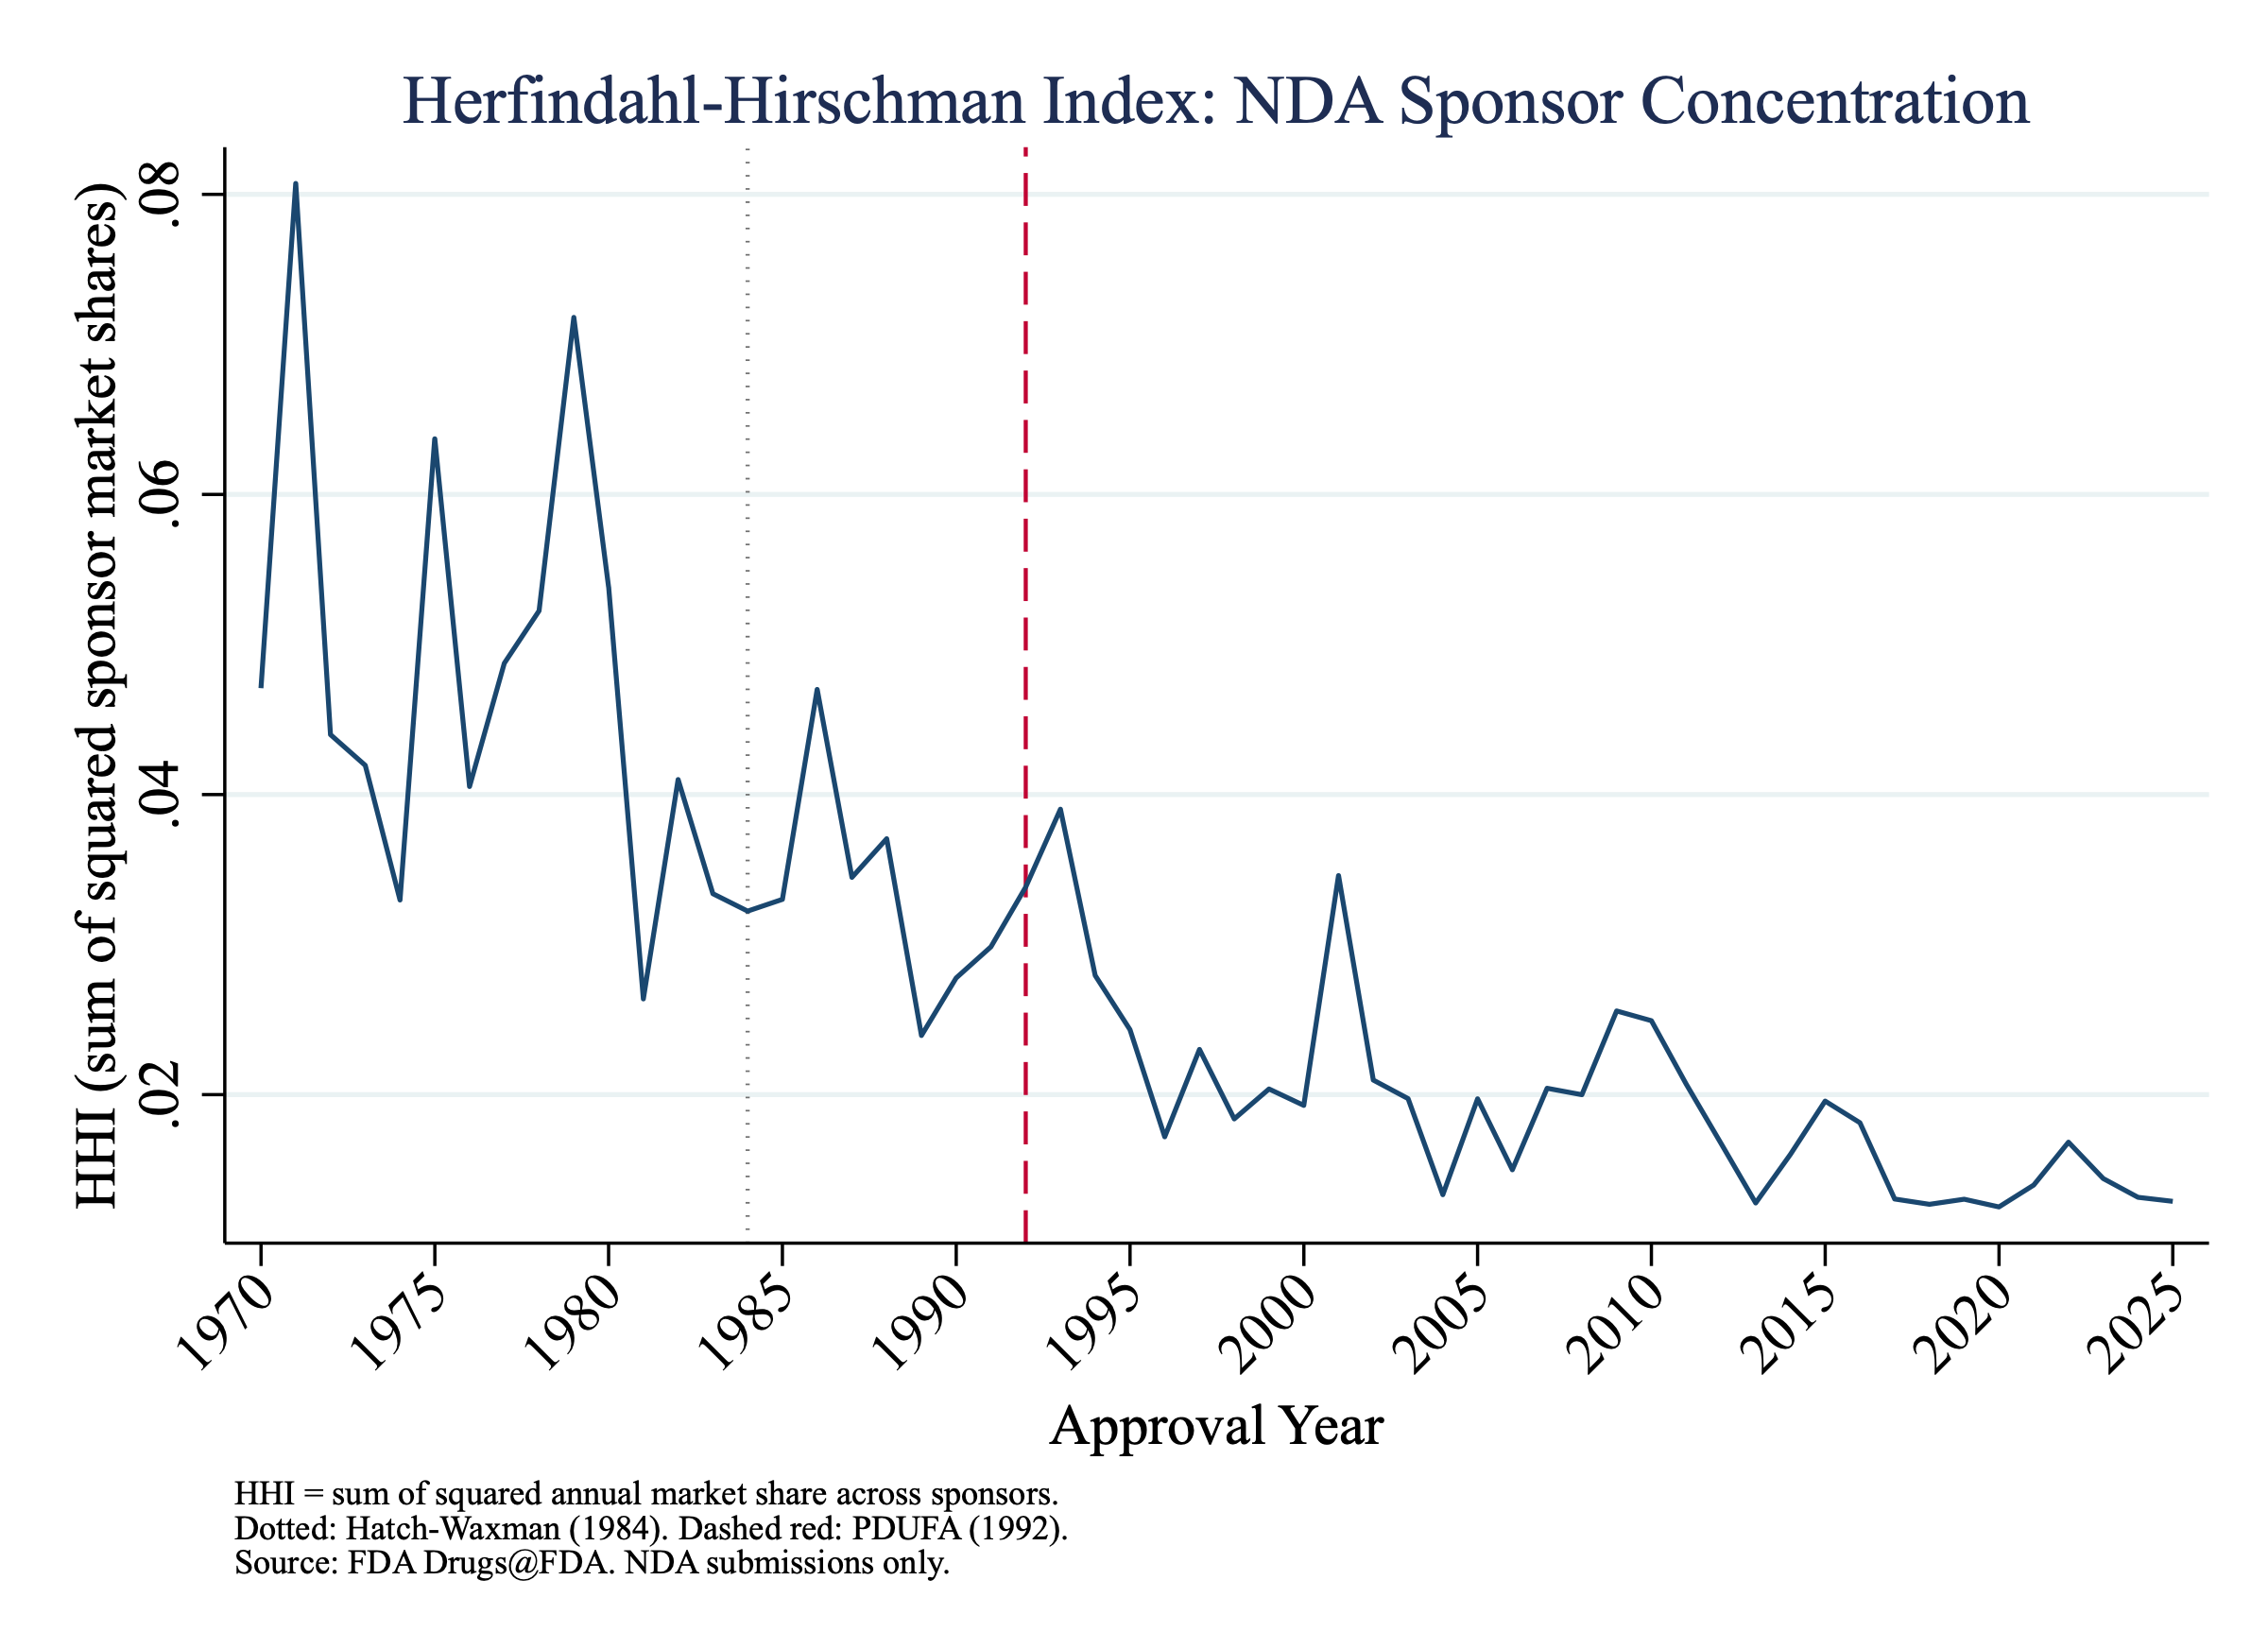
\includegraphics[width=0.92\textwidth]{../output/figures/stata/pdufa_nda_sponsor_concentration_hhi.png}
\caption{Sponsor HHI for CS NDA approvals, 1970--2025. Higher HHI = greater sponsor concentration. PDUFA reference lines marked.}
\label{fig:nda_hhi}
\end{figure}

\begin{figure}[htbp]
\centering
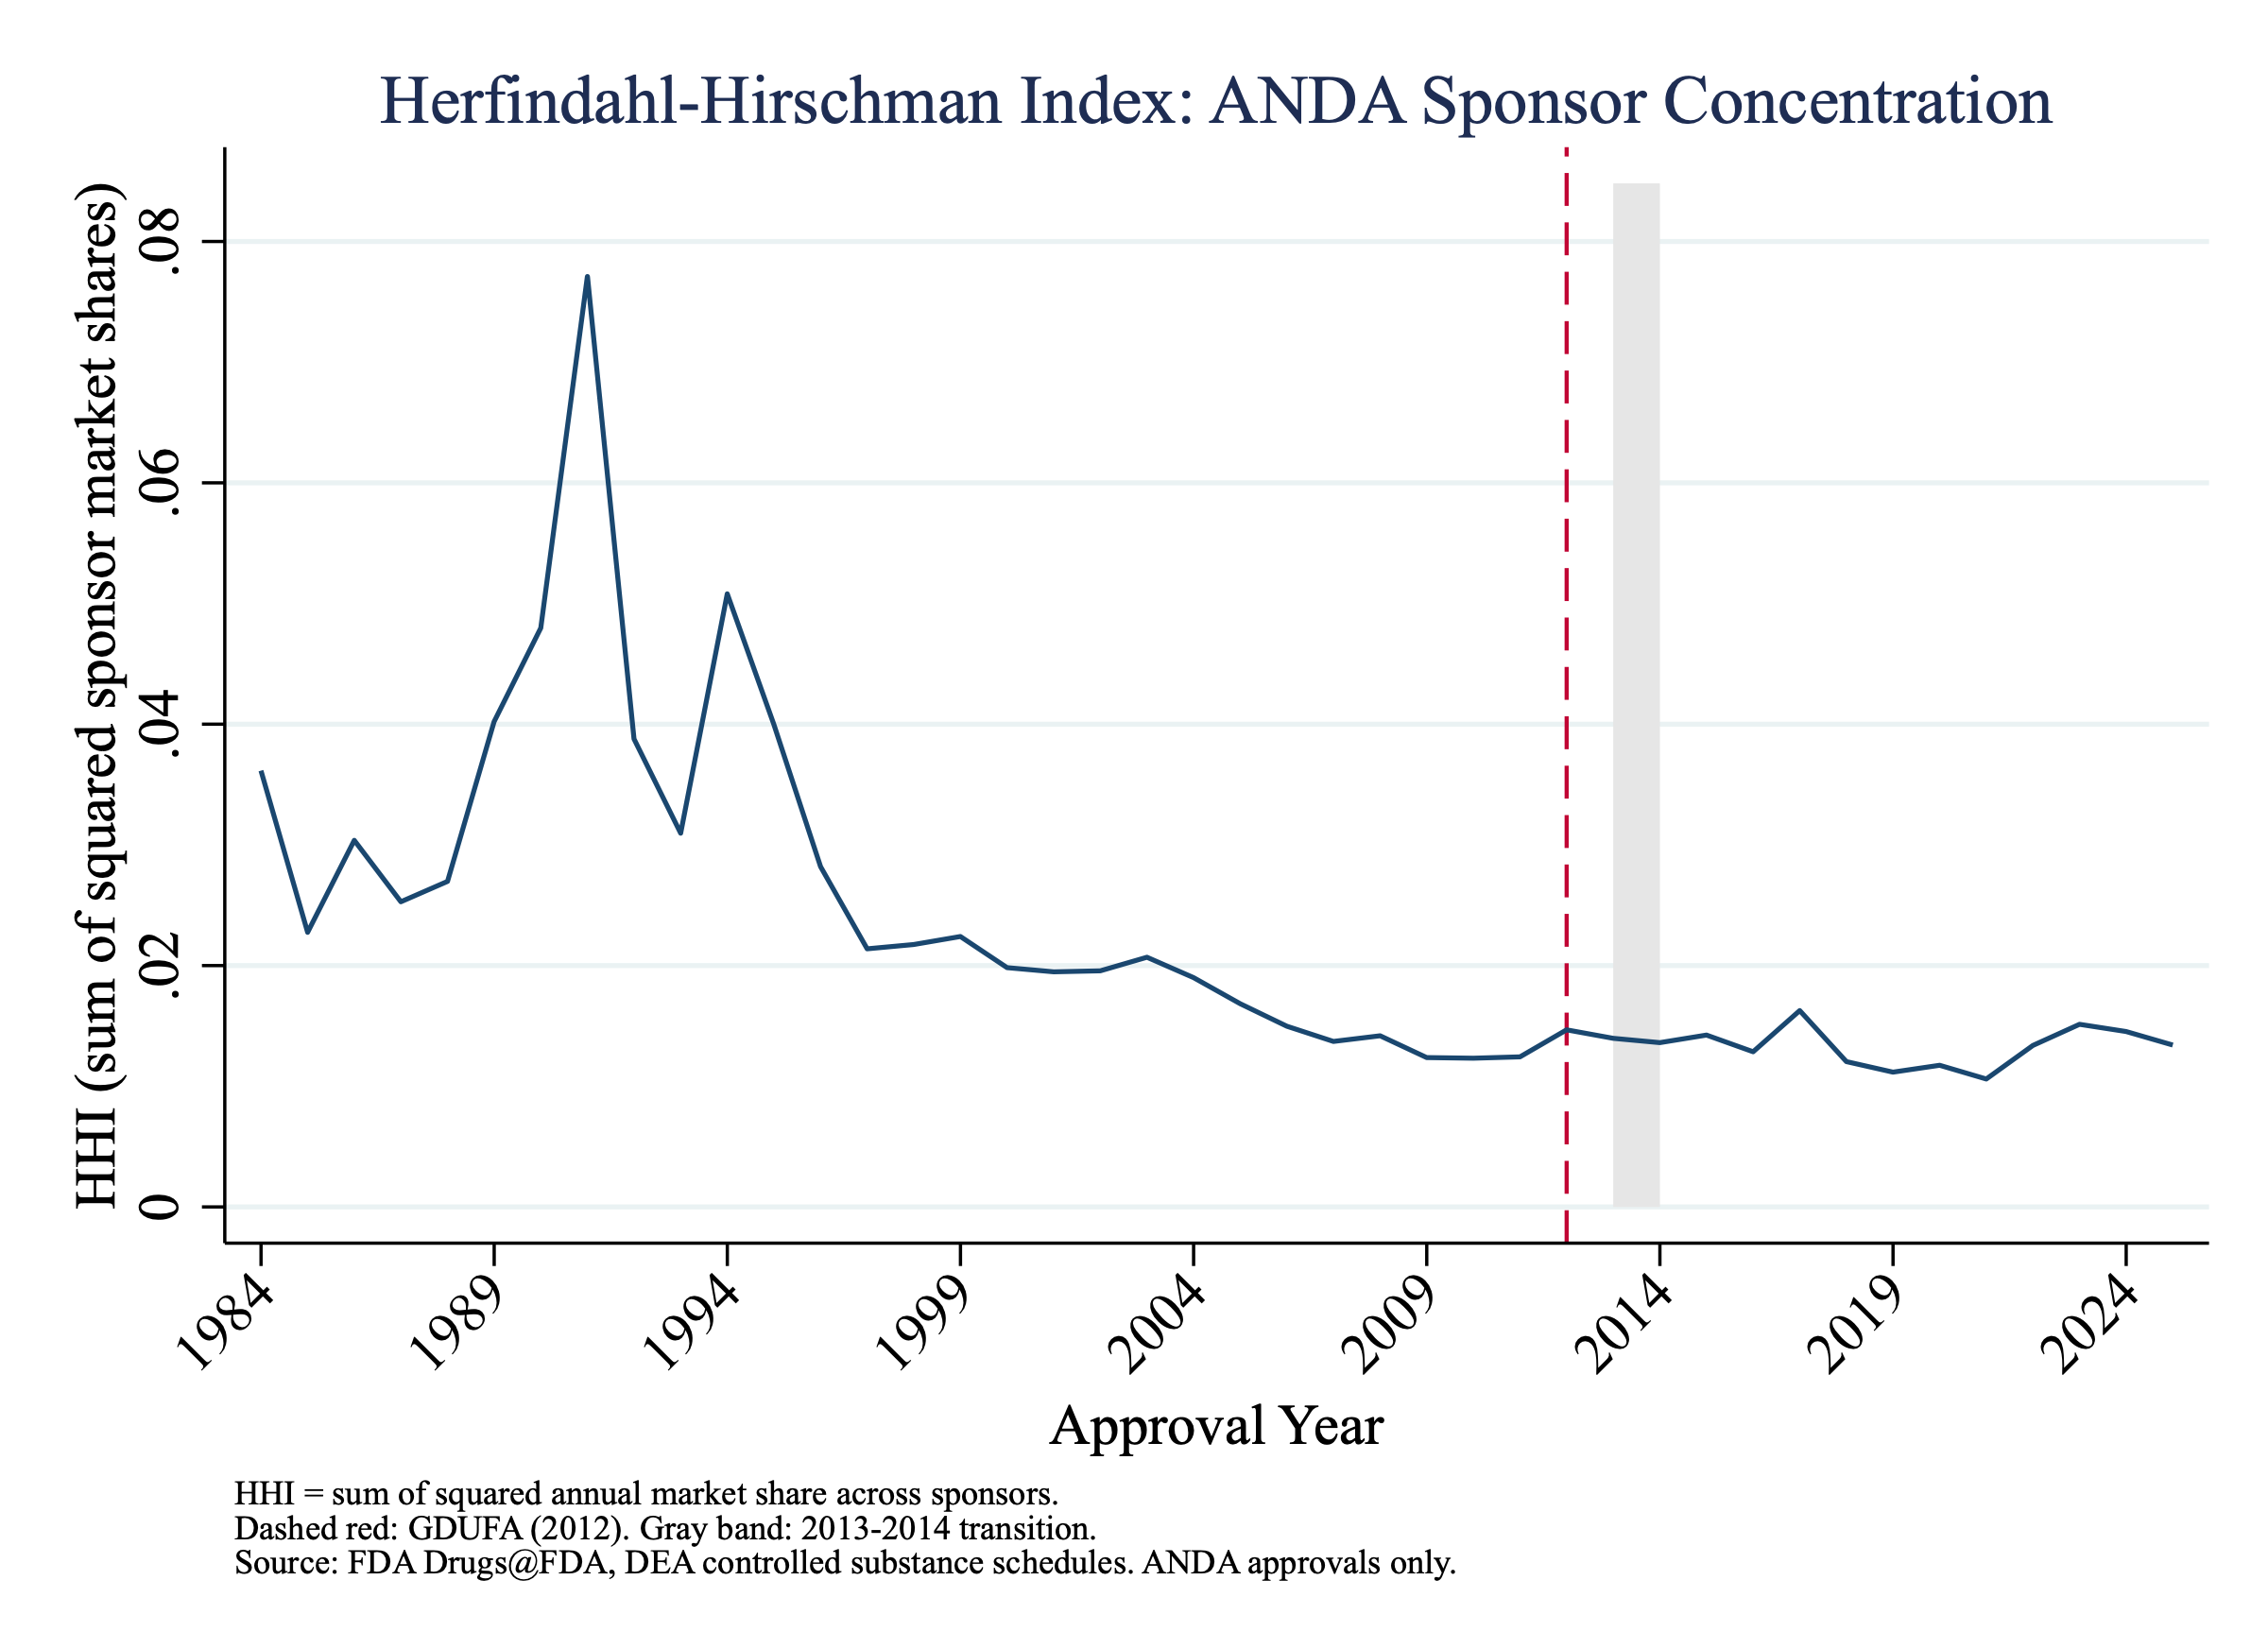
\includegraphics[width=0.92\textwidth]{../output/figures/stata/gdufa_sponsor_concentration_hhi.png}
\caption{Sponsor HHI for ANDA approvals (all), 1984--2025. GDUFA reference line marked.}
\label{fig:gdufa_hhi}
\end{figure}

Table~\ref{tab:top_sponsors} reports the top sponsors of CS NDA approvals over the full 1970--2025 period. The market is fragmented: the leading sponsors (HIKMA and UCB INC, tied at 9 CS NDAs each) account for only 4.1\% of the 222 CS NDAs in this window. Purdue Pharma LP ranks fourth with 7 approvals (3.2\%), reflecting both its historical dominance in branded opioid formulations and the relatively small absolute scale of any single sponsor's CS NDA portfolio.

\begin{table}[htbp]
\centering
\begin{threeparttable}
\caption{Top 10 Sponsors of CS NDA Approvals, 1970--2025}
\label{tab:top_sponsors}
\small
\begin{tabular}{llrr}
\toprule
Rank & Sponsor & CS NDAs & Share (\%) \\
\midrule
1 & HIKMA & 9 & 4.05 \\
1 & UCB INC & 9 & 4.05 \\
3 & SPECGX LLC & 7 & 3.15 \\
3 & PURDUE PHARMA LP & 7 & 3.15 \\
5 & INDIVIOR & 5 & 2.25 \\
5 & SANOFI AVENTIS US & 5 & 2.25 \\
5 & UPJOHN & 5 & 2.25 \\
8 & ABBOTT & 4 & 1.80 \\
8 & COLLEGIUM PHARM INC & 4 & 1.80 \\
8 & JANSSEN PHARMS & 4 & 1.80 \\
8 & TAKEDA PHARMS USA & 4 & 1.80 \\
\bottomrule
\end{tabular}
\begin{tablenotes}
\footnotesize
\item Universe: CS NDAs with confident DEA schedule match, 1970--2025, sponsor name non-missing.
\item Total CS NDAs in window: 222. Source: \texttt{cs\_nda\_top\_sponsors\_1970\_2025.csv}.
\end{tablenotes}
\end{threeparttable}
\end{table}
